\section{实验}
实验结果按以下方式呈现：首先在\S\ref{detail}中详细说明数据集、评估指标和实现细节；然后在\S\ref{sota}中将本文方法与现有工作进行对比；在\S\ref{overlap}中评估不同模型在相机重叠区域的性能；在\S\ref{pseudo}中与前向预测模型进行比较；最后在\S\ref{ablation}中提供额外的分析和消融实验。

\subsection{实现细节}
\label{detail}

\textbf{数据集（Dataset）。} 在nuScenes数据集~\cite{nuscenes2019}上进行测试。nuScenes包含1,000个序列，每个序列长约20秒，采样率为20帧/秒。每个样本包含6个相机图像 \texttt{[front\_left, front, front\_right, back\_left, back, back\_right]}。提供了包括内参和外参在内的相机参数。nuScenes每0.5秒提供一次标注，训练集、验证集和测试集分别有28k、6k和6k个标注样本。从全部23个类别中选取10个类别用于计算评估指标。

\textbf{评估指标（Metrics）。} 遵循nuScenes提供的官方评估协议。评估平均平移误差（Average Translation Error, ATE）、平均尺度误差（Average Scale Error, ASE）、平均朝向误差（Average Orientation Error, AOE）、平均速度误差（Average Velocity Error, AVE）和平均属性误差（Average Attribute Error, AAE）。这些指标是真正例指标（True Positive Metrics, TP Metrics），以物理单位计算。此外，还测量平均精度（mean Average Precision, mAP）。为全面捕获检测任务的所有方面，定义了一个综合标量指标——nuScenes检测得分（nuScenes Detection Score, NDS）~\cite{nuscenes2019}：$\mathrm{NDS} = \frac{1}{10}[5\mathrm{mAP}+\sum_{\mathrm{mTP}\in \mathbb{TP}}(1-\min(1, \mathrm{mTP}))]$。
% \begin{equation}
%     \begin{split}
%     \mathrm{NDS} = \frac{1}{10}[5\mathrm{mAP}+\sum_{\mathrm{mTP}\in \mathbb{TP}}(1-\min(1, \mathrm{mTP}))].
%     \end{split}
% \end{equation}

\textbf{模型（Model）。} 本文模型由ResNet~\cite{He2015}特征提取器、FPN和\name 检测头组成。使用在第3和第4阶段具有可变形卷积~\cite{dai17dcn}的ResNet101。FPN~\cite{Lin2017}接收ResNet输出的特征，生成4张尺寸分别为输入图像大小$\nicefrac18$、$\nicefrac1{16}$、$\nicefrac1{32}$和$\nicefrac1{64}$的特征图。\name 检测头包含6层，每层由一个特征优化步骤和一个多头注意力层组成。\name 检测头的隐藏维度为256。最后，两个子网络分别预测每个目标查询的边界框参数和类别标签；每个子网络由两个隐藏维度为256的全连接层组成。在检测头中使用层归一化（LayerNorm）~\cite{BaKH16}。

\textbf{训练与推理（Training \& Inference）。} 使用AdamW~\cite{loshchilov2018decoupled}训练整个流程。权重衰减为$10^{-4}$。初始学习率为$10^{-4}$，在第8和第11个epoch分别降至$10^{-5}$和$10^{-6}$。模型总共训练12个epoch，使用8张RTX 3090 GPU，每GPU批大小为1。训练过程大约需要18小时。推理时不使用NMS等后处理。评估使用nuScenes评估工具包。

\subsection{与现有工作对比}
\label{sota}
与之前的当前最优方法CenterNet~\cite{zhou2019centernet}和FCOS3D~\cite{wang2021fcos3d}进行比较。CenterNet是一种无锚框2D检测方法，在高分辨率特征图上进行密集预测。FCOS3D采用FCOS~\cite{tian2019fcos}流程进行逐像素预测。这两种方法都将3D目标检测转化为2D问题，因此忽略了场景几何和传感器配置。为执行多视角目标检测，这些方法必须独立处理每张图像，并分别使用逐图像和全局NMS来去除各视角和重叠区域中的冗余框。如表~\ref{table:sota}所示，本文方法即使不使用任何后处理，也优于这些方法。本文方法在mATE指标上略逊于FCOS3D，推测是因为FCOS3D直接预测边界框深度，从而对目标平移提供了强监督。此外，FCOS3D为不同的边界框参数使用了解耦检测头，这有助于提升性能。

在测试集上（表~\ref{table:sota:test}），截至2021年10月13日，本文方法优于所有现有方法；为公平比较，本文方法与DD3D~\cite{dd3d}使用相同的骨干网络。

\begin{table}[t] 
\begin{center}
\caption{在验证集上与近期工作的对比。本文方法对NMS的使用具有鲁棒性。$\ast$：CenterNet使用自定义骨干网络DLA~\cite{Yu_2018_CVPR}。$\ddag$：该模型使用深度权重1.0训练，并从FCOS3D检查点初始化；该检查点在同一数据集上使用深度权重0.2训练。$\S$：使用测试时数据增强。$\P$：使用测试时数据增强、更多epoch和模型集成。详见\cite{wang2021fcos3d}。$\dag$：本文方法同样从FCOS3D骨干网络初始化；检测头随机初始化。$\#$：使用CBGS~\cite{cbgs}训练。\label{table:sota}}
\vspace{-1.0em}
\resizebox{\linewidth}{!}{
\begin{tabular}{c|c|c|c|c|c|c|c|c}
\toprule
\hline
方法 & NDS $\uparrow$ & mAP $\uparrow$ & mATE $\downarrow$ & mASE $\downarrow$ & mAOE $\downarrow$ & mAVE $\downarrow$ & mAAE $\downarrow$ & NMS \\
\hline
CenterNet  $\ast$ & 0.328 & 0.306 & 0.716 & 0.264 & 0.609 & 1.426 & 0.658 & \checkmark \\
\hline
FCOS3D  & 0.373 & 0.299 & 0.785 & 0.268 & 0.557 & 1.396 & 0.154 & \checkmark \\
\hline
\changed{FCOS3D $\ddag$} & \changed{0.393} & \changed{0.321} & \changed{0.746} & \changed{0.265} & \changed{0.503} & \changed{1.351} & \changed{0.160} & \changed{\checkmark} \\

\hline

\changed{FCOS3D $\S$} & \changed{0.402} & \changed{0.326} & \changed{0.743} & \changed{0.259} & \changed{0.441} & \changed{1.341} & \changed{0.163} & \changed{\checkmark} \\

\hline

\changed{FCOS3D $\P$} & \changed{0.415} & \changed{0.343} & \changed{0.725} & \changed{0.263} & \changed{0.422} & \changed{1.292} & \changed{0.153} & \changed{\checkmark} \\

\hline

\name (Ours)   &  0.374 & 0.303 & 0.860 & 0.278 & 0.437 & 0.967 & 0.235 & - \\
\hline
\changed{\name (Ours) $\dag$} & \changed{0.425} & \changed{0.346} & \changed{0.773} & \changed{0.268} & \changed{0.383} & \changed{0.842} & \changed{0.216} & \changed{-} \\
\hline

\changed{\name (Ours) $\#$} & 0.434 & 0.349 & 0.716 & 0.268 & 0.379 & 0.842 & 0.200 & - \\
\hline

\bottomrule
\end{tabular}
}
\end{center}
\end{table}


\begin{table}[t] 
\begin{center}
\caption{在测试集上与排行榜上最优方法的对比。\label{table:sota:test} $\#$：从DD3D检查点初始化。$\dag$：从额外数据预训练的骨干网络初始化。}
\vspace{-0.5em}
\resizebox{\linewidth}{!}{
\begin{tabular}{c|c|c|c|c|c|c|c|c}
\toprule
\hline
方法 & NDS $\uparrow$ & mAP $\uparrow$ & mATE $\downarrow$ & mASE $\downarrow$ & mAOE $\downarrow$ & mAVE $\downarrow$ & mAAE $\downarrow$ & NMS \\
\hline 
Mono3D & 0.429 & 0.366 & 0.642 & 0.252 & 0.523 & 1.591 & 0.119 & N/A \\ 
\hline 
DHNet & 0.437 & 0.363 & 0.667 & 0.259 & 0.402 & 1.589 & 0.120 & N/A \\ 
\hline 
PGD~\cite{wang2021probabilistic} & 0.448 & 0.386 & 0.626 & 0.245 & 0.451 & 1.509 & 0.127 & \checkmark \\ 
\hline
DD3D~\cite{dd3d} $\dag$ & 0.477 & 0.418 & 0.572 & 0.249 & 0.368 & 1.014 & 0.124 & \checkmark \\
\hline
\name (Ours) $\#$ & 0.479 & 0.412 & 0.641 & 0.255 & 0.394 & 0.845 & 0.133 & - \\
\hline
\bottomrule
\end{tabular}
}
\end{center}
\end{table}


\subsection{重叠区域对比}
\label{overlap}
重叠区域是一个巨大挑战，因为目标更容易被截断。本文方法同时考虑所有相机，而FCOS3D则逐相机独立预测边界框。为进一步展示融合推理的优势，计算落入相机重叠区域的边界框的评估指标。具体而言，选择3D中心被多个相机可见的框。在验证集上，共有18,147个这样的框，占总数的9.7%。表~\ref{table:overlap}展示了结果；在该设置下，本文方法在NDS得分上显著优于FCOS3D。这证实了集成预测方法更加有效。

\begin{table}[t] 
\begin{center}
% \vspace{-1.0em}
\caption{重叠区域对比。$\ddag$：该模型使用深度权重1.0训练，并从FCOS3D检查点初始化；该检查点在同一数据集上使用深度权重0.2训练。详见\cite{wang2021fcos3d}。$\dag$：本文方法同样从FCOS3D骨干网络初始化；检测头随机初始化。\label{table:overlap}}
% \vspace{-1.0em}
\resizebox{\linewidth}{!}{
\begin{tabular}{c|c|c|c|c|c|c|c|c}
\toprule
\hline
方法 & NDS $\uparrow$ & mAP $\uparrow$ & mATE $\downarrow$ & mASE $\downarrow$ & mAOE $\downarrow$ & mAVE $\downarrow$ & mAAE $\downarrow$ & NMS \\
\hline
\hline
FCOS3D & 0.317 & 0.213 & 0.841 & 0.276 & 0.604 & 1.122 & 0.173 &  \checkmark \\
\hline
\changed{FCOS3D}$\ddag$ & \changed{0.329} & \changed{0.229} & \changed{0.816} & \changed{0.272} & \changed{0.571} & \changed{1.084} & \changed{0.195} &  \changed{\checkmark} \\
\hline
\name (Ours)  &  0.356 & 0.231 & 0.825 & 0.280 & 0.400 & 0.863 & 0.223 & - \\
\hline
\changed{\name (Ours)} $\dag$ &  \changed{0.384} & \changed{0.268} & \changed{0.807} & \changed{0.273} & \changed{0.453} & \changed{0.788} & \changed{0.184} & \changed{-} \\
\hline
\bottomrule
\end{tabular}
}
\end{center}
% \vspace{-2.5em}
\end{table}


\subsection{与伪激光雷达方法对比}
\label{pseudo}
另一种执行3D目标检测的方式是使用深度预测模型从多视角图像生成伪激光雷达点云。在nuScenes数据集上，没有公开可用的伪激光雷达工作可供直接比较。因此，自行实现一个基线方法以验证本文方法优于显式深度预测。使用预训练的PackNet~\cite{packnet}网络从所有六个相机预测密集深度图，然后使用相机变换将这些深度图转换为点云。还尝试了带有速度监督的自监督PackNet模型（如原始论文所述），但发现真值深度监督能生成更真实的点云，因此使用有监督模型作为基线。对于3D检测，采用最近提出的CenterPoint架构~\cite{yin2021center}。从概念上讲，该流程是伪激光雷达（Pseudo-LiDAR）~\cite{wang2019pseudo}的一个变体。表~\ref{pseudolidar}展示了结果；即使深度估计由当前最优模型生成，该伪激光雷达方法仍显著不如本文方法。一个可能的解释是，伪激光雷达目标检测器受到不准确深度预测引入的累积误差的影响，而深度预测本身容易过拟合训练数据且对其他数据分布泛化能力差~\cite{demistifying}。%, while our approach does not use depth at all.%<--- debatable  
% \vitor{Are there any published Pseudo-LiDAR methods that we can also use as comparison? It would make this part more convincing, right now feels like we just came up with something to compare and outperformed it, there is no weight to that}

\begin{table}[t] 
\begin{center}
\caption{与伪激光雷达方法对比。\label{pseudolidar}}
\vspace{-1em}
\resizebox{\linewidth}{!}{
\begin{tabular}{c|c|c|c|c|c|c|c|c}
\toprule
\hline
方法 & NDS $\uparrow$ & mAP $\uparrow$ & mATE $\downarrow$ & mASE $\downarrow$ & mAOE $\downarrow$ & mAVE $\downarrow$ & mAAE $\downarrow$ & NMS \\
\hline
pseudo-LiDAR & 0.160 & 0.048 & - & - & - & - & - & \checkmark \\
\hline
\name (Ours)  &  0.374 & 0.303 & 0.860 & 0.278 & 0.437 & 0.967 & 0.235 & - \\
\hline
\bottomrule
\end{tabular}
}
\end{center}
  \vspace{-0.8em}
\end{table}

\subsection{消融实验与分析}
\label{ablation}

图~\ref{fig:iter-refine}可视化了目标查询的优化过程。可视化了每一层从目标查询解码出的边界框。随着模型层数加深，预测边界框逐渐逼近真值。左侧子图展示了从所有数据中学习到的共享目标查询先验。表~\ref{tab:ablation}提供了定量结果，表明迭代优化确实显著提升了性能。这表明迭代优化对于充分利用本文提出的架构既有益又必要。此外，表~\ref{tab:queries}提供了目标查询数量的消融实验；增加查询数量持续提升性能，直到在900个查询时饱和。最后，表~\ref{tab:backbone}展示了不同骨干网络的结果。

\begin{table}[t] 
\begin{center}
  \vspace{-0.8em}
\caption{不同层检测结果的评估。\label{tab:ablation}}
%   \vspace{-0.8em}
\resizebox{0.8\linewidth}{!}{
\begin{tabular}{c|c|c|c|c|c|c|c}
\toprule
\hline
层数 $\uparrow$ & NDS $\uparrow$ & mAP $\uparrow$ & mATE $\downarrow$ & mASE $\downarrow$ & mAOE $\downarrow$ & mAVE $\downarrow$ & mAAE $\downarrow$  \\
\hline
0 & \changed{0.380} & \changed{0.302}  & \changed{0.855} & \changed{0.280} & \changed{0.435} & \changed{0.910} & \changed{0.231}  \\
\hline
1  &  \changed{0.410} & \changed{0.335} & \changed{0.791} & \changed{0.275} & \changed{0.408} & \changed{0.887} & \changed{0.217} \\
\hline
2  & \changed{0.420} & \changed{0.343} & \changed{0.782} & \changed{0.271} & \changed{0.395} & \changed{0.851} & \changed{0.214} \\
\hline
3  & \changed{0.420} & \changed{0.346} & \changed{0.778} & \changed{0.268} & \changed{0.390} & \changed{0.874} & \changed{0.218} \\
\hline
4  &  \changed{0.424} & \changed{0.346} & \changed{0.777} & \changed{0.268} & \changed{0.389} & \changed{0.855} & \changed{0.217} \\
\hline
5  &  \changed{0.425} & \changed{0.346} & \changed{0.773} & \changed{0.268} & \changed{0.383} & \changed{0.842} & \changed{0.216} \\
\hline
\bottomrule
\end{tabular}
}
\end{center}
  \vspace{-0.8em}
\end{table}

\begin{figure}[t!]  
  \vspace{-0.8em}
    \centering
    \begin{tabular}{@{}ccc@{}}
        第1层 & 第2层 & 第3层 \\
        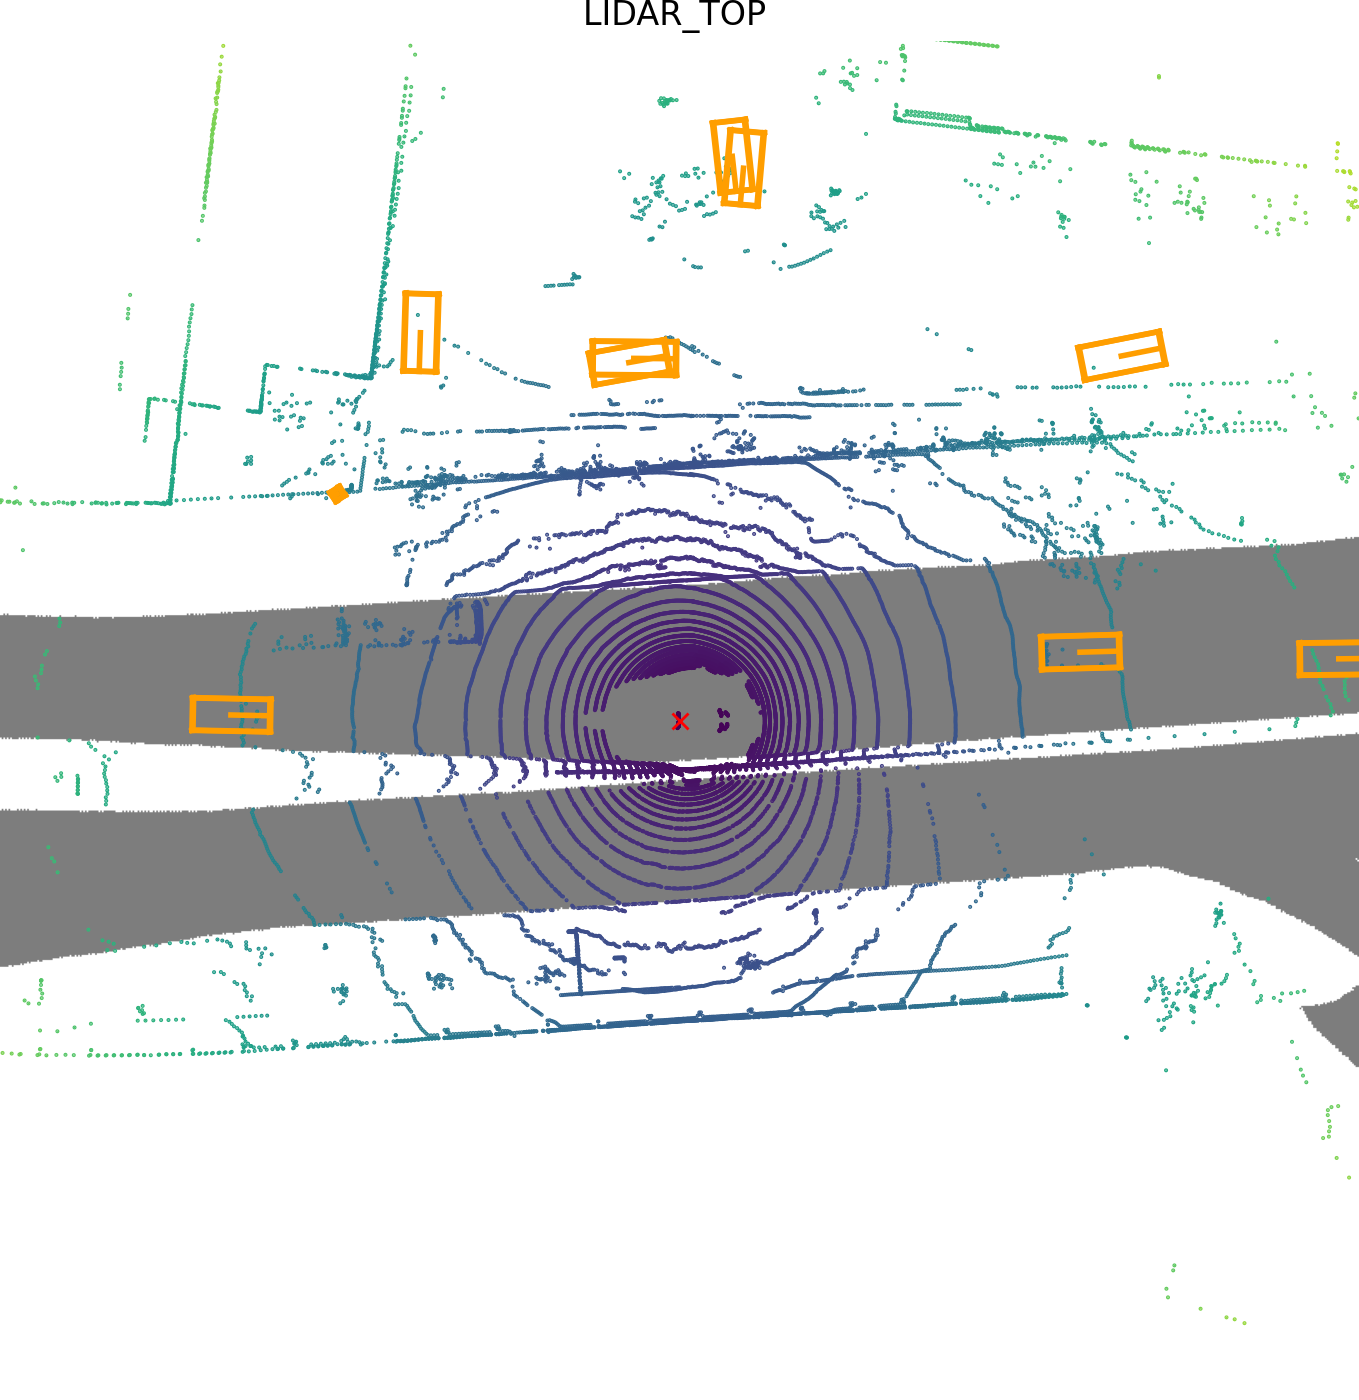
\includegraphics[width=0.31\columnwidth]{figure/iterative_refine_bev/level0.png} & 
    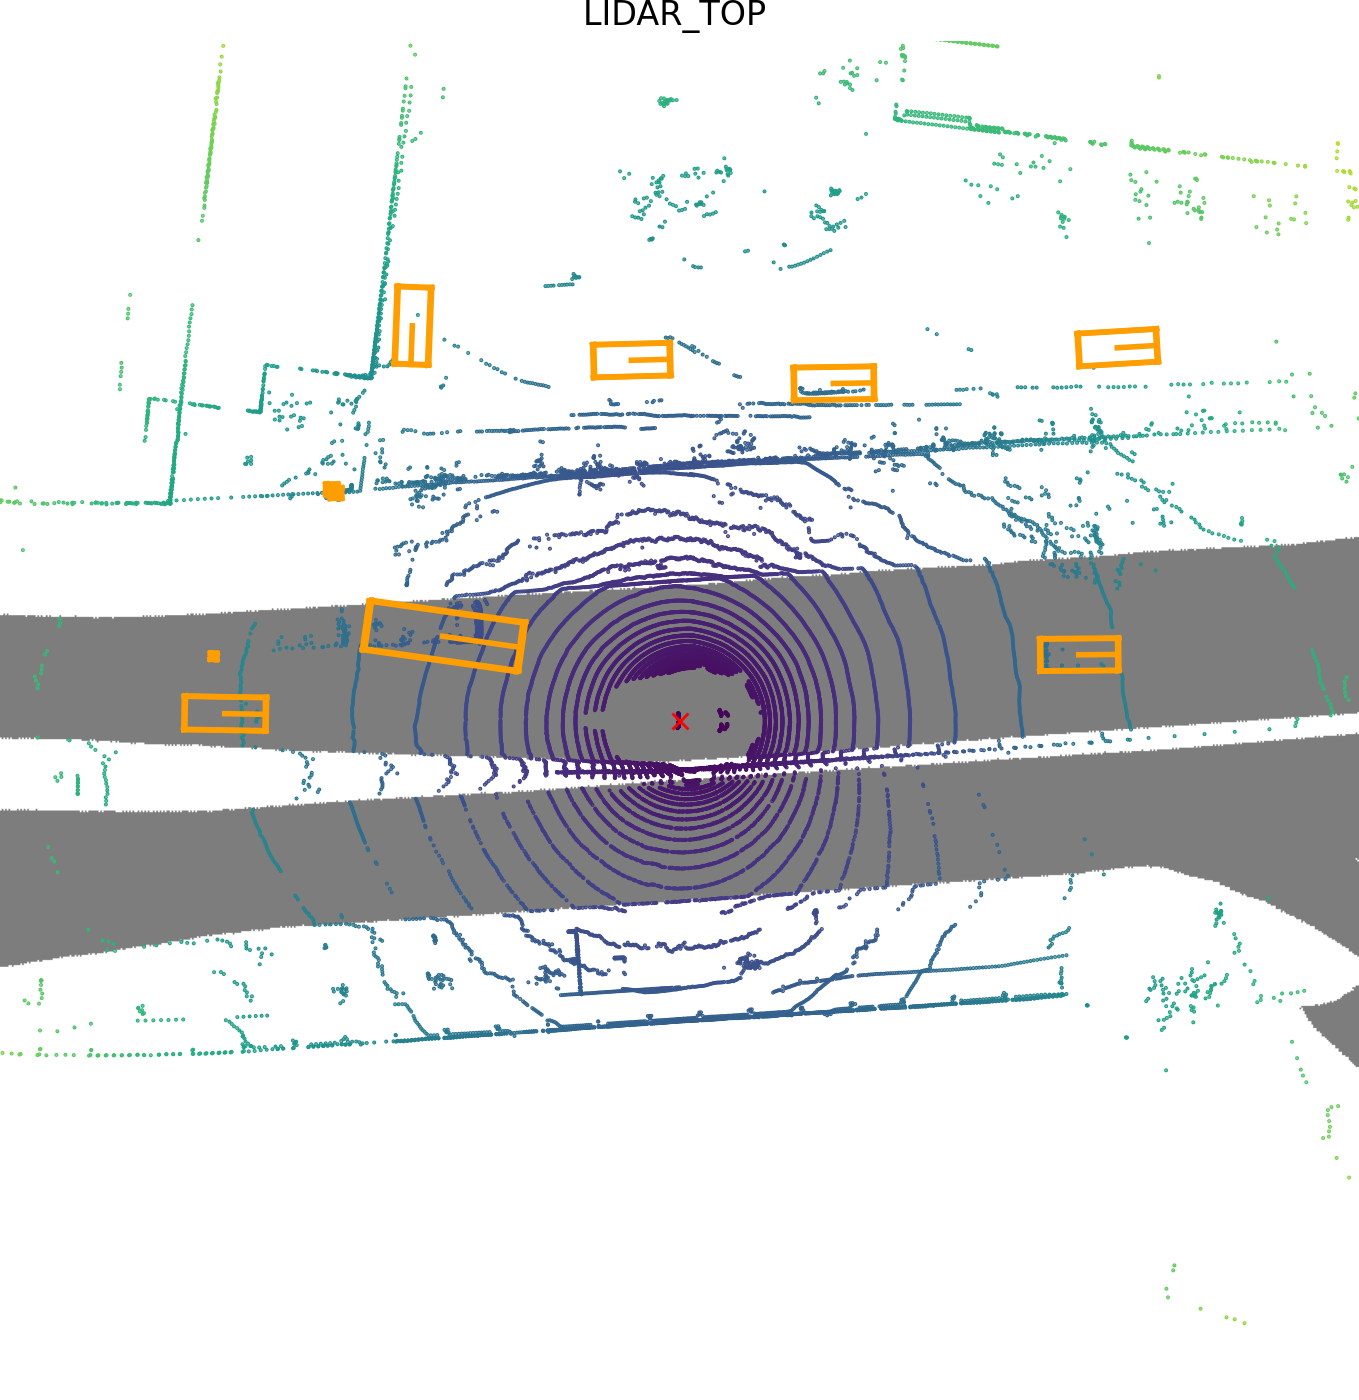
\includegraphics[width=0.31\columnwidth]{figure/iterative_refine_bev/level1.png} &
    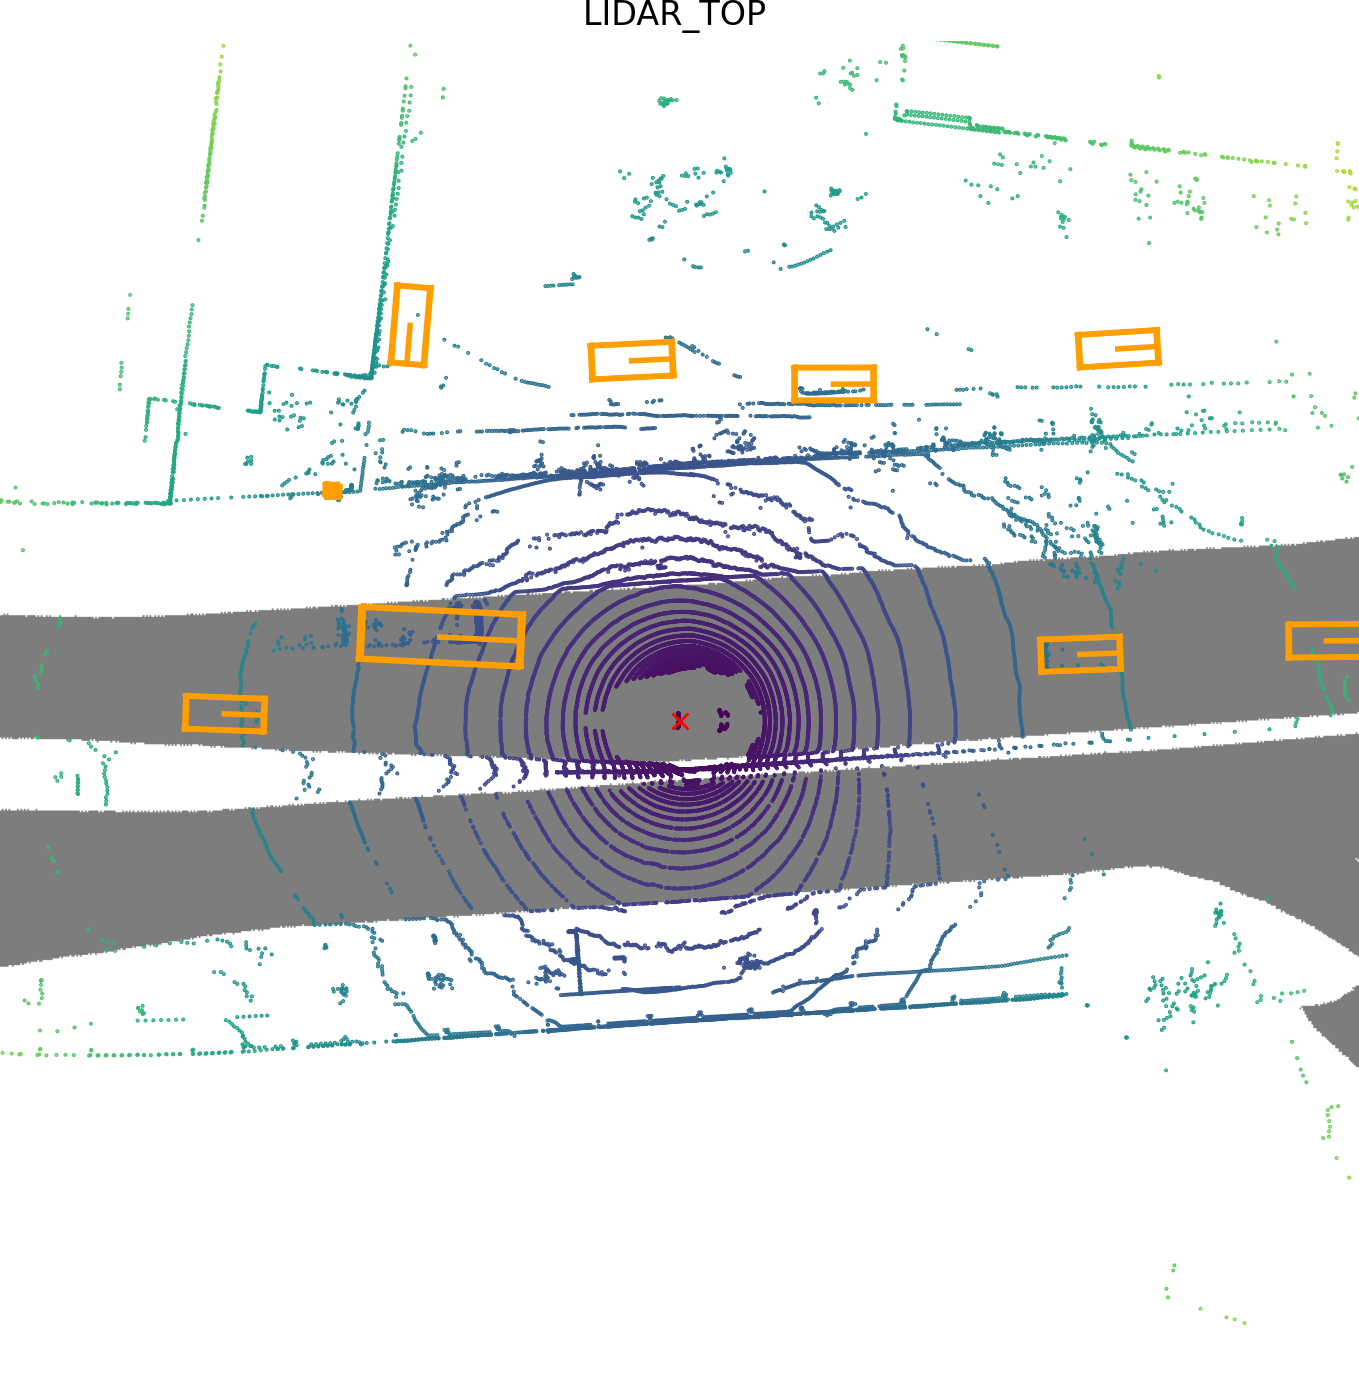
\includegraphics[width=0.31\columnwidth]{figure/iterative_refine_bev/level2.png} \\
        第4层 & 第5层 & 真值 \\
    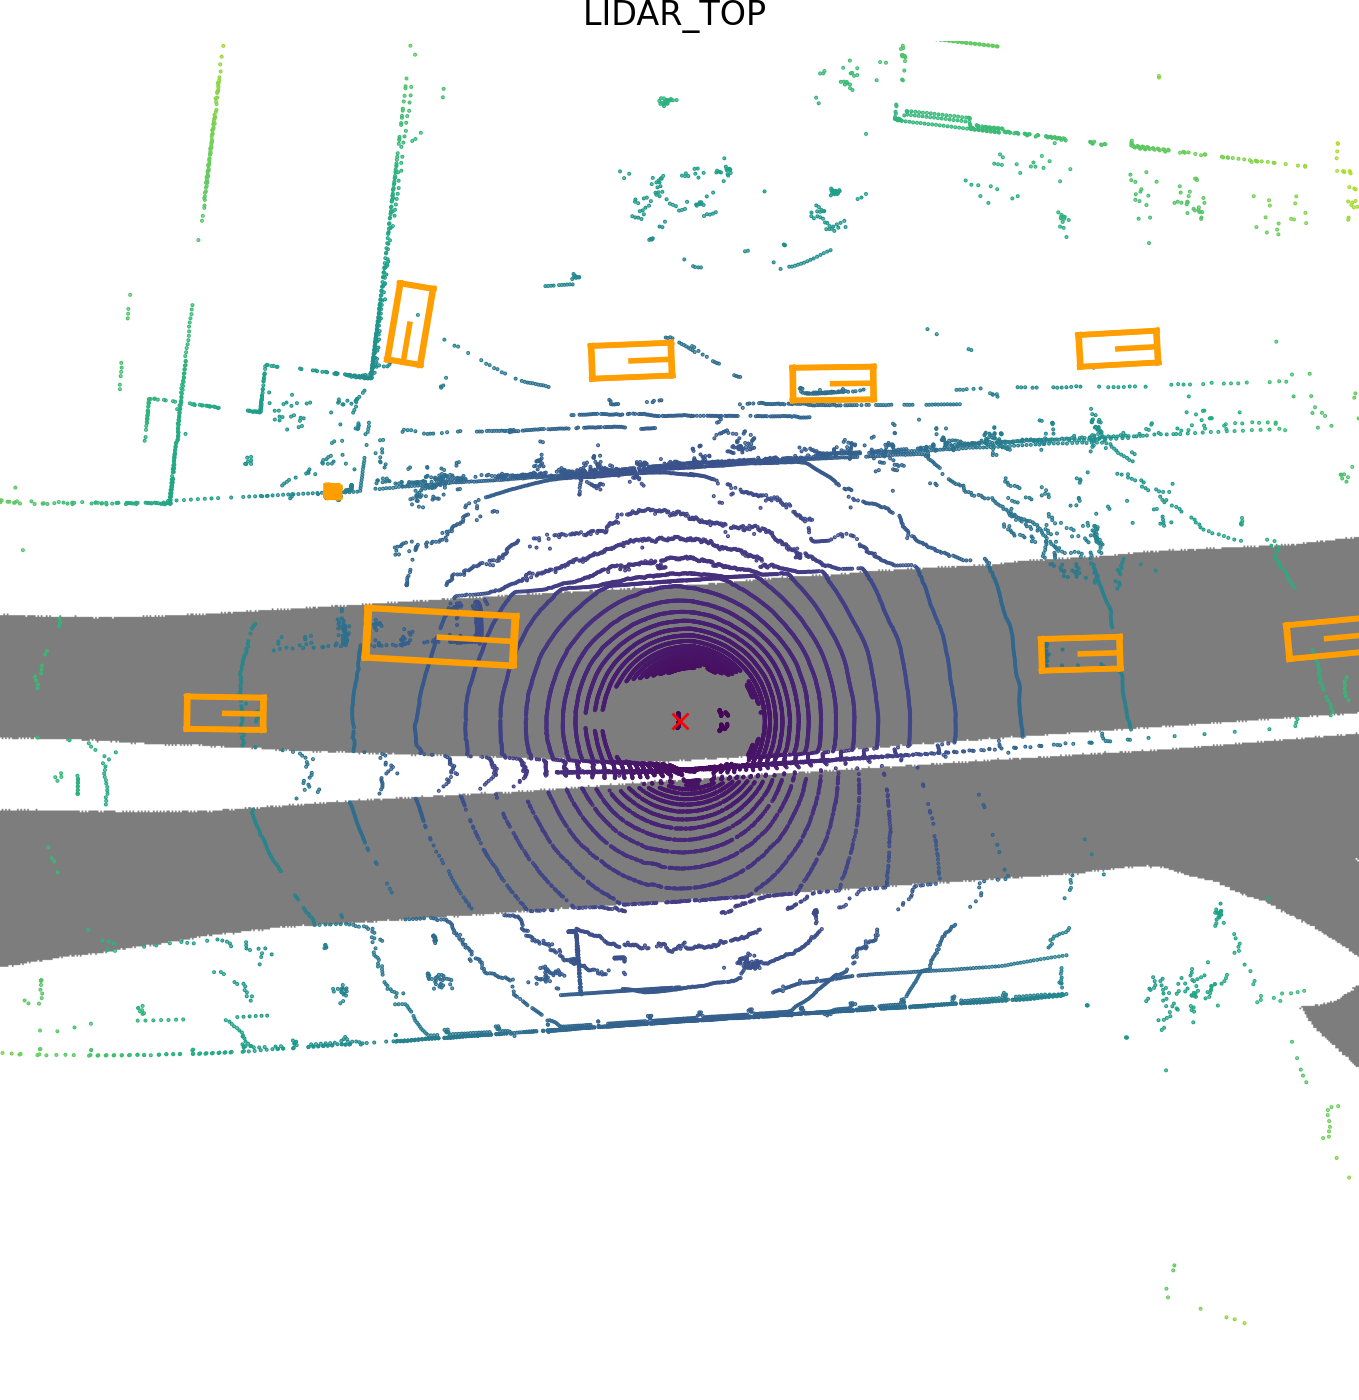
\includegraphics[width=0.31\columnwidth]{figure/iterative_refine_bev/level3.png} & 
    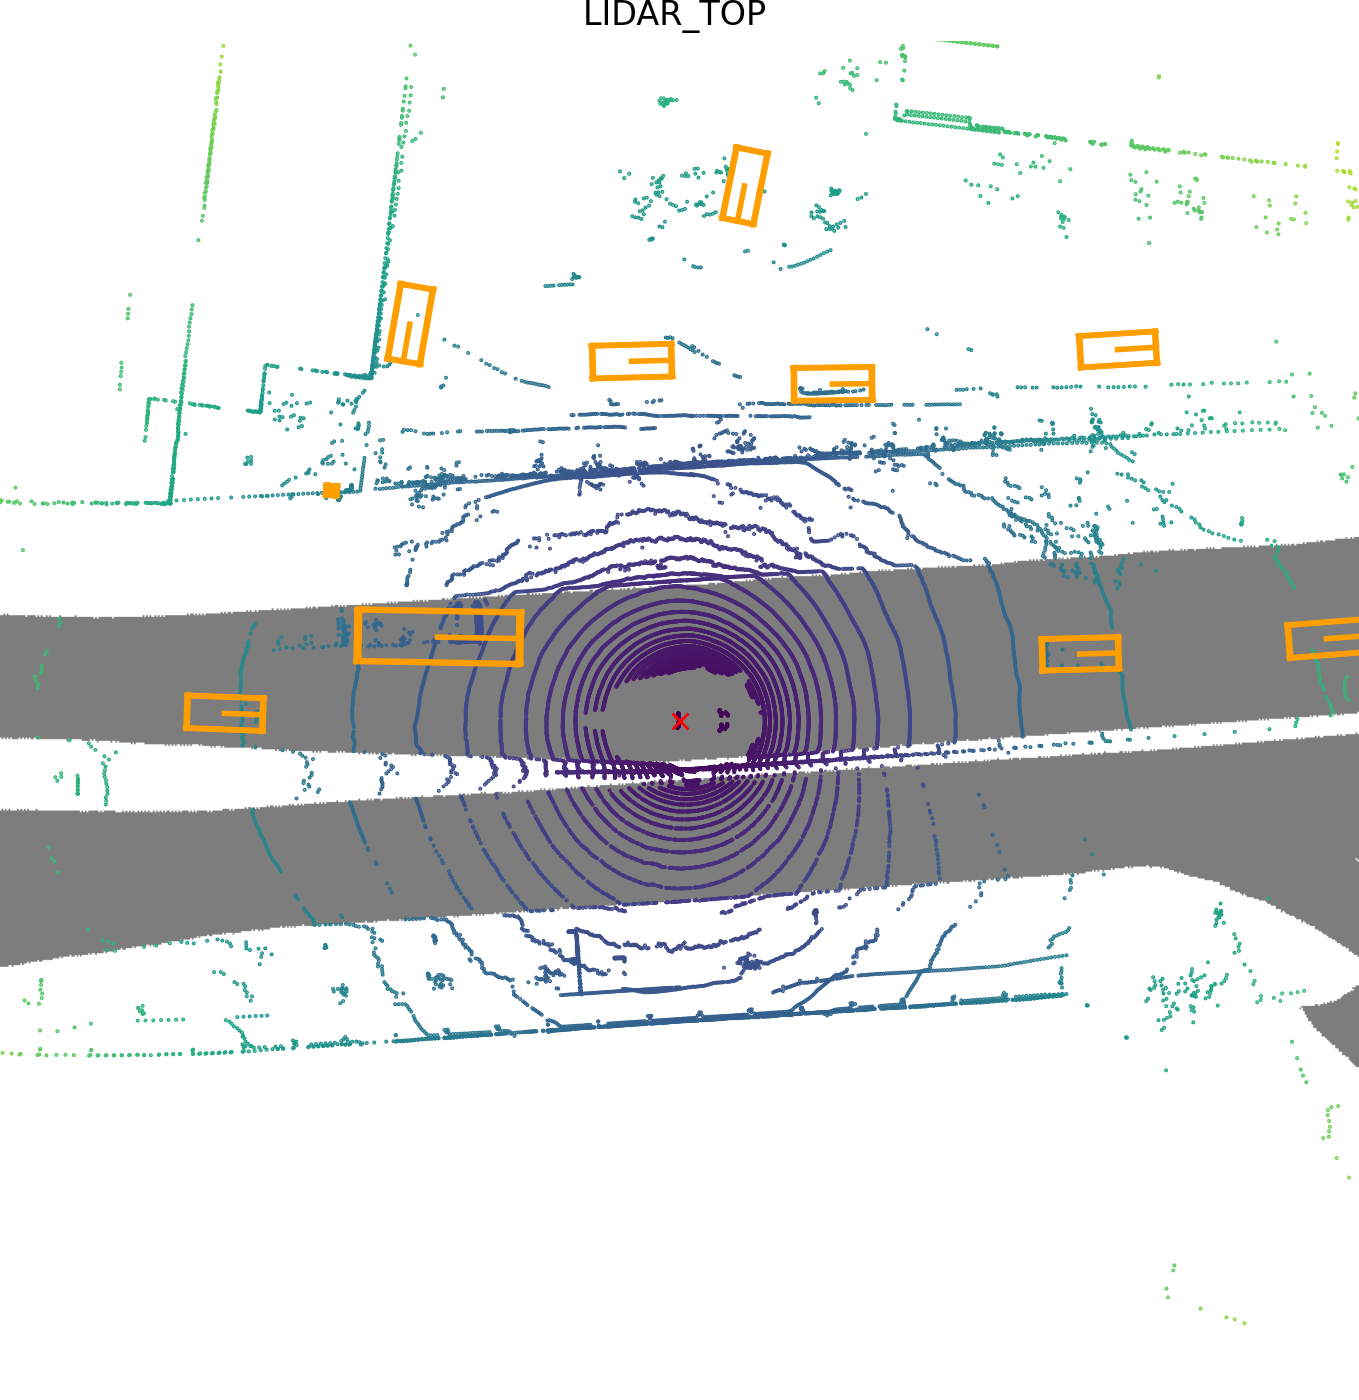
\includegraphics[width=0.31\columnwidth]{figure/iterative_refine_bev/level4.png} & 
        \includegraphics[width=0.31\columnwidth]{figure/iterative_refine_bev/GT-LIDAR_TOP.png} 
    \end{tabular}
%   \vspace{-2.5em}
  \caption{\name 头中第1层到第5层的检测结果。在BEV中可视化边界框，并叠加来自\texttt{lidar\_top}的点云。随着层数加深，预测逐渐接近真值。\label{fig:iter-refine}}
%   \vspace{-2em}
\end{figure}

\begin{table}[t] 
\begin{center}
%   \vspace{-0.8em}
\caption{不同查询数量的结果。\label{tab:queries}}
\resizebox{0.8\linewidth}{!}{
\begin{tabular}{c|c|c|c|c|c|c|c}
\toprule
\hline
\changed{查询数量} & \changed{30} & \changed{100} & \changed{300} & \changed{600} & \changed{900} & \changed{1200} & \changed{1500}  \\
\hline
\changed{mAP $\uparrow$} & \changed{0.201} & \changed{0.313} & \changed{0.338} & \changed{0.347} & \changed{0.346} & \changed{0.340} & \changed{0.346}  \\
\hline
\changed{NDS $\uparrow$} & \changed{0.331} & \changed{0.408} & \changed{0.415} & \changed{0.420} & \changed{0.425} & \changed{0.415} & \changed{0.420}  \\
\bottomrule
\end{tabular}
}
\end{center}
\end{table}

\begin{table}[ht] 
\begin{center}
  \vspace{-1em}
\caption{不同骨干网络的结果。\label{tab:backbone}}
\resizebox{0.8\linewidth}{!}{
\begin{tabular}{c|c|c|c|c|c|c|c}
\toprule
\hline
\changed{骨干网络 $\uparrow$} & \changed{NDS $\uparrow$} & \changed{mAP $\uparrow$} & \changed{mATE $\downarrow$} & \changed{mASE $\downarrow$} & \changed{mAOE $\downarrow$} & \changed{mAVE $\downarrow$} & \changed{mAAE $\downarrow$}  \\
\hline
\changed{ResNet50} & \changed{0.373} & \changed{0.302} & \changed{0.811} & \changed{0.282} & \changed{0.493} & \changed{0.979} & \changed{0.212}  \\
\hline
\changed{ResNet101} & \changed{0.425} & \changed{0.346} & \changed{0.773} & \changed{0.268} & \changed{0.383} & \changed{0.842} & \changed{0.216}\\
\hline
\changed{DLA34} & \changed{0.394} & \changed{0.312} & \changed{0.829} & \changed{0.276} & \changed{0.450} & \changed{0.844} & \changed{0.221} \\
\hline
\bottomrule
\end{tabular}
}
\end{center}
  \vspace{-1em}

\end{table}

图~\ref{fig:prediction}还提供了定性结果，以便直观理解模型性能。将预测的边界框投影到6个相机视图以及BEV视角中。总体而言，本文方法生成了合理的结果，甚至能检测到相对较小的目标。然而，本文方法仍然存在显著的平移误差（与表~\ref{sota}的结果一致）：尽管模型避免了显式深度预测，深度估计仍然是该问题的核心挑战。

% \begin{comment}
\begin{figure}[t!]  
\renewcommand{\arraystretch}{2}

    \centering
    \begin{tabular}{@{}cc@{}}
    \begin{minipage}{.27\textwidth}
        \begin{tabular}{@{}p{1em}@{}c@{}}
        \rotatebox{90}{\small{预测}} & 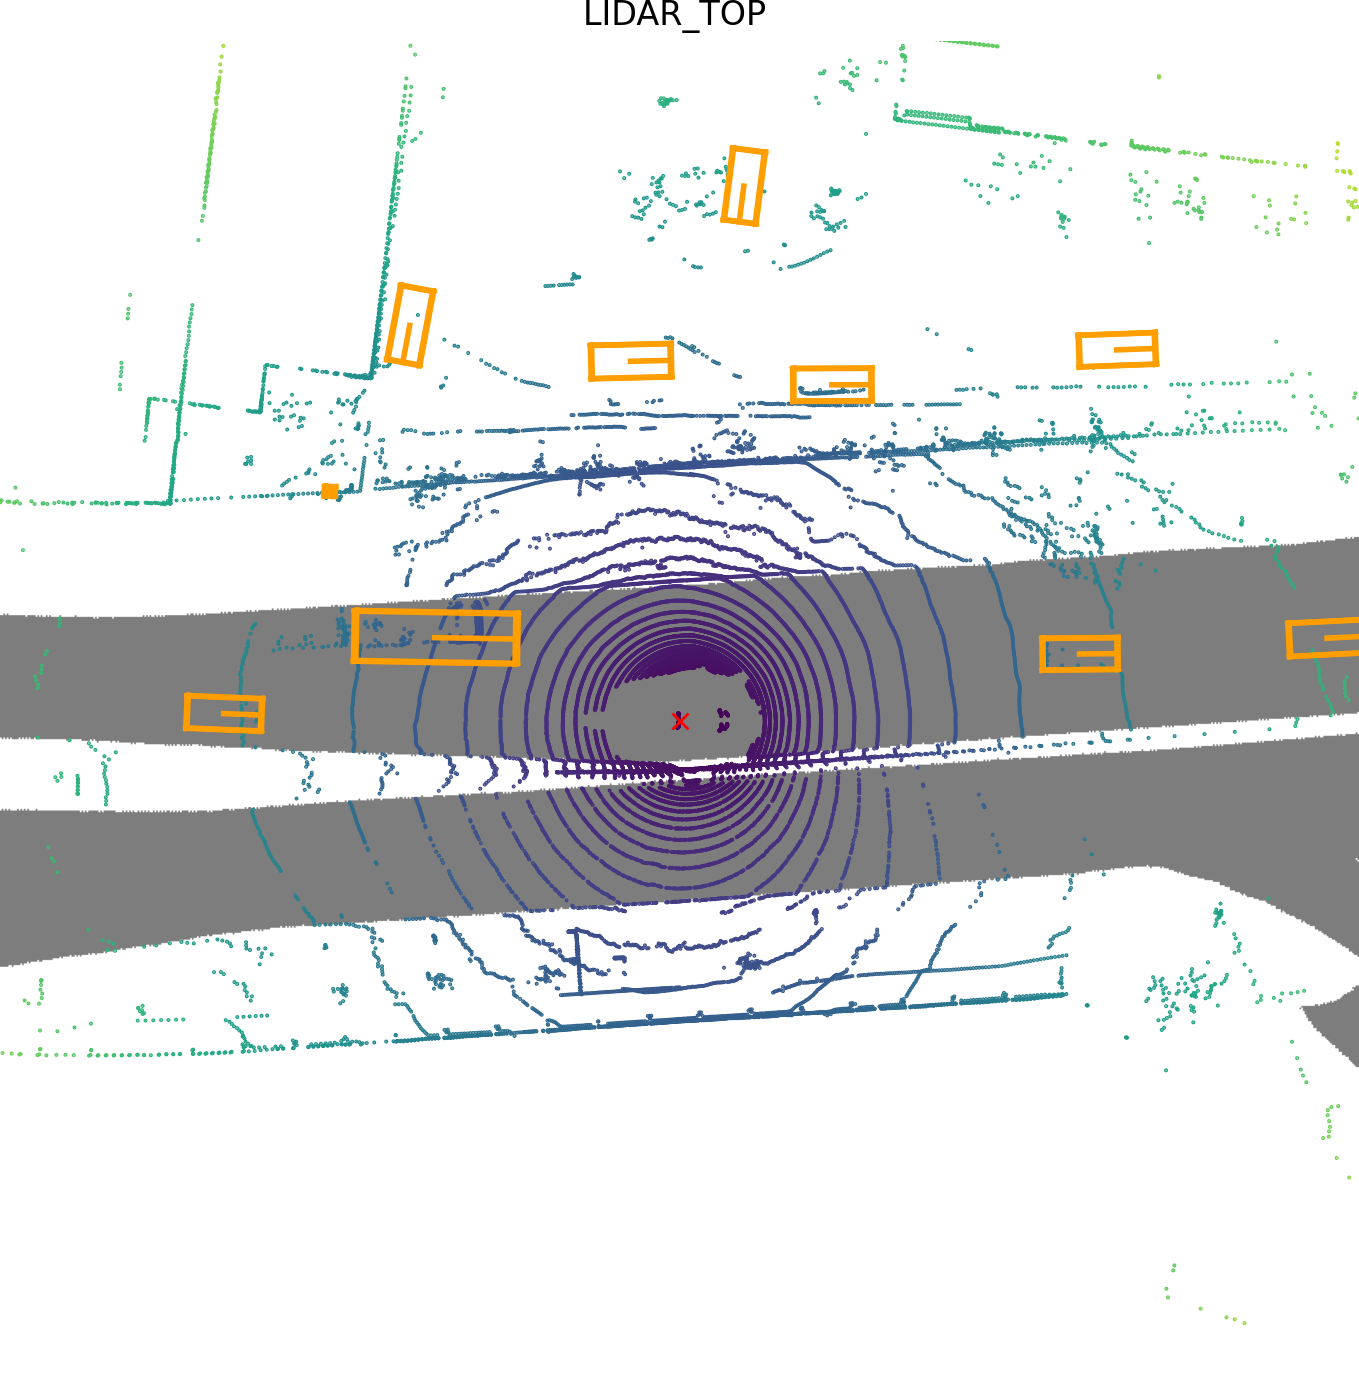
\includegraphics[width=1.0\textwidth]{figure/visualize_predictions/LIDAR_TOP.png}
    \end{tabular}
    \end{minipage}
    & 
    \begin{minipage}{.73\textwidth}
        \begin{tabular}{@{}p{1em}@{}c@{}c@{}c@{}}
        \centering \rotatebox{90}{\small{预测}} &
    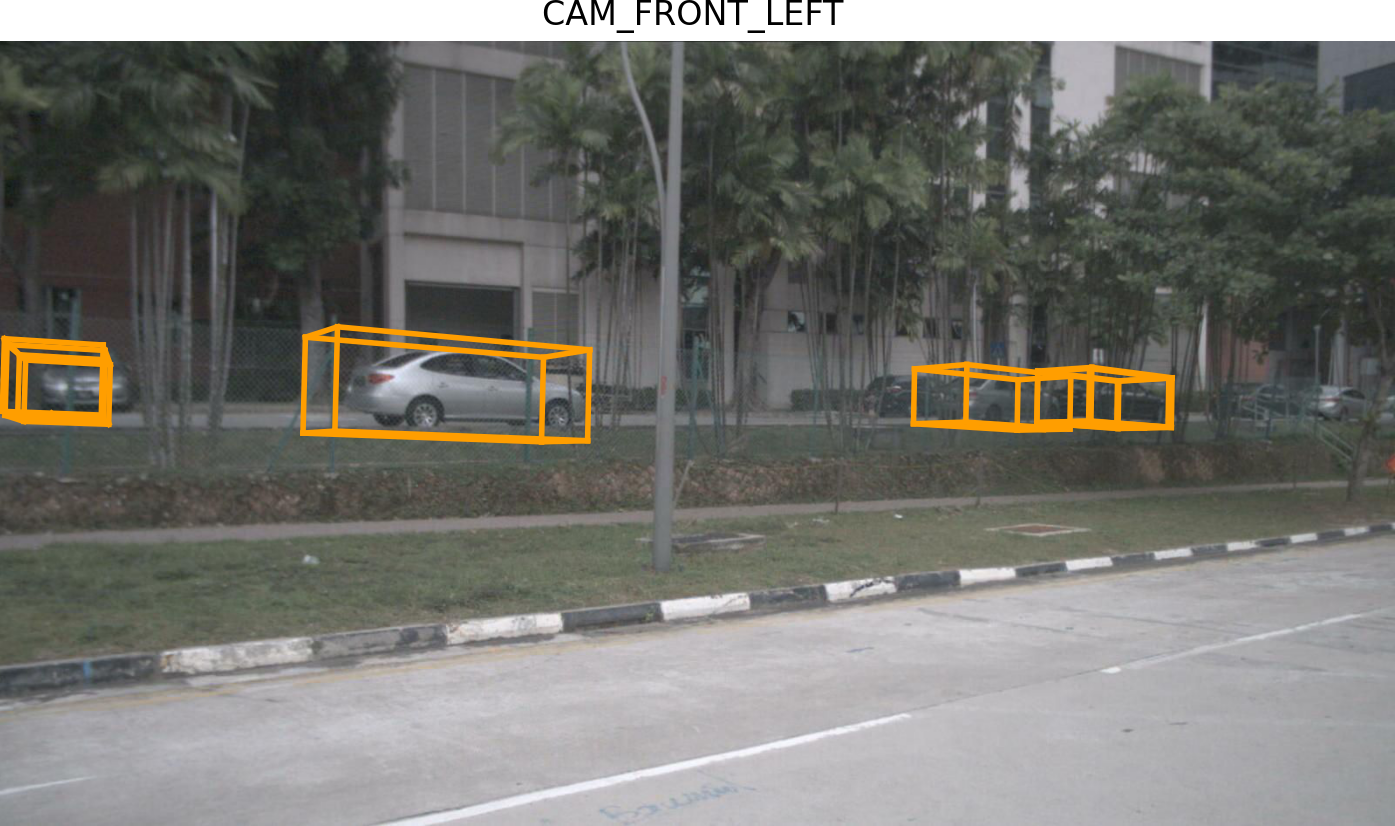
\includegraphics[width=0.31\columnwidth]{figure/visualize_predictions/CAM_FRONT_LEFT.png} & 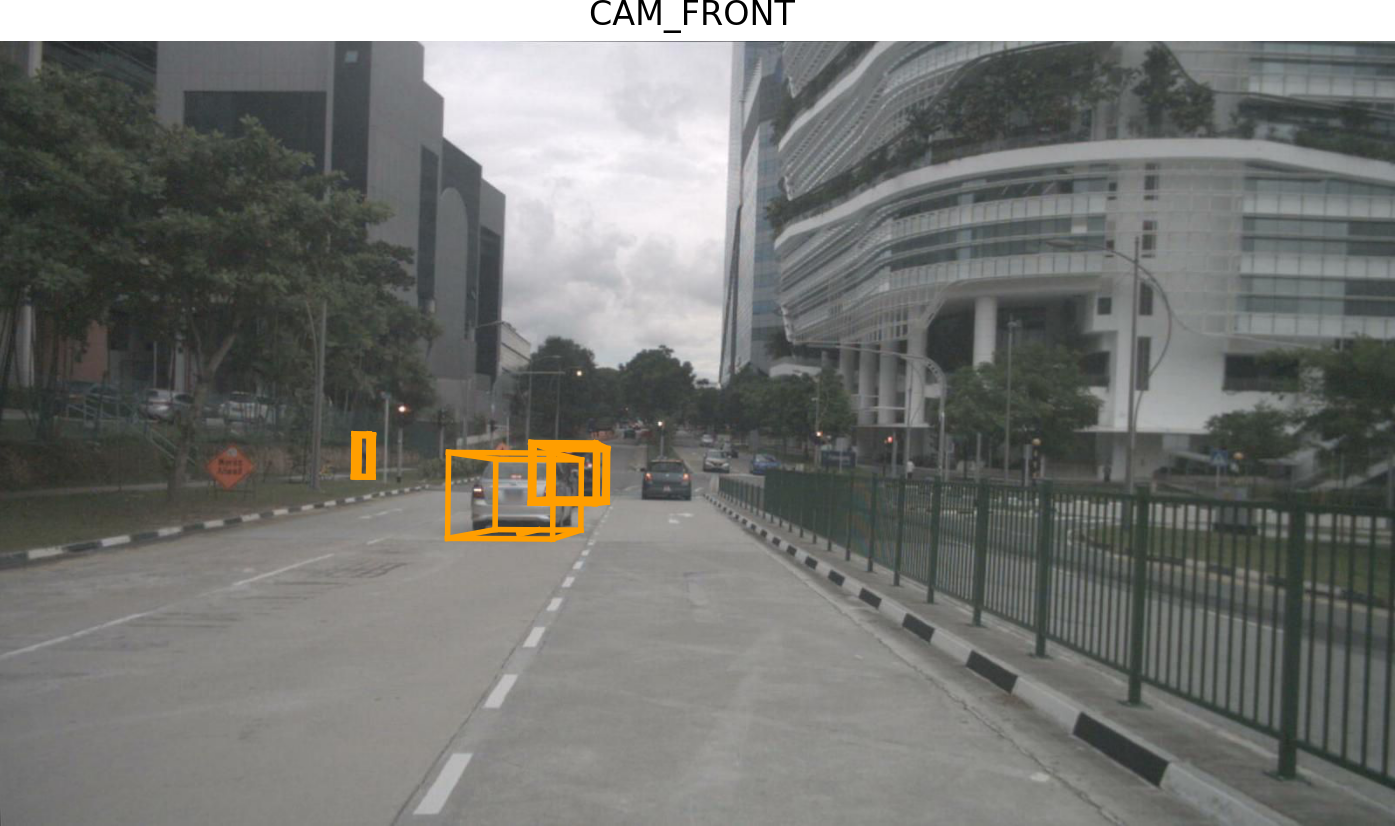
\includegraphics[width=0.31\columnwidth]{figure/visualize_predictions/CAM_FRONT.png} & 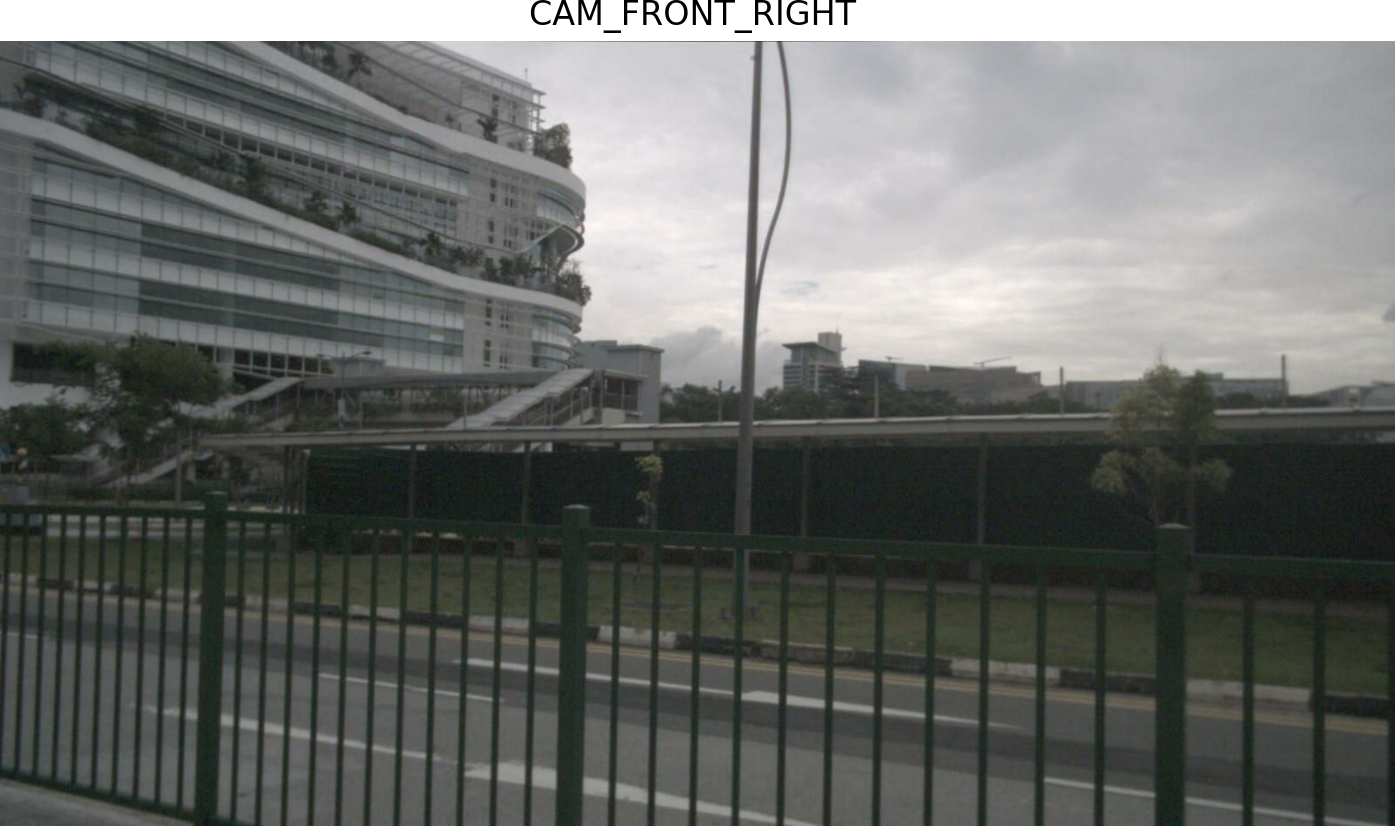
\includegraphics[width=0.31\columnwidth]{figure/visualize_predictions/CAM_FRONT_RIGHT.png} \\ 
            \rotatebox{90}{\small{真值}} &
    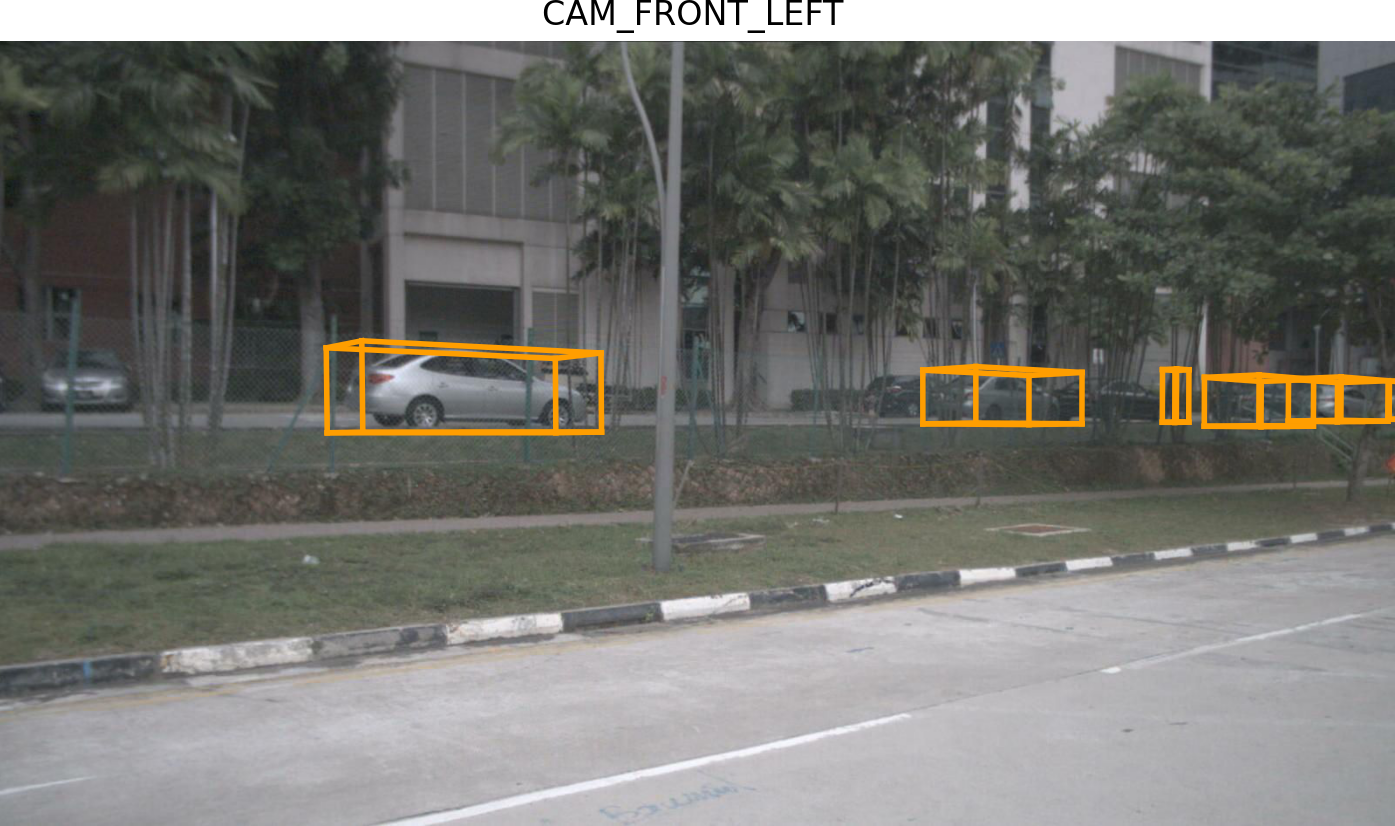
\includegraphics[width=0.31\columnwidth]{figure/visualize_predictions/GT-CAM_FRONT_LEFT.png} & 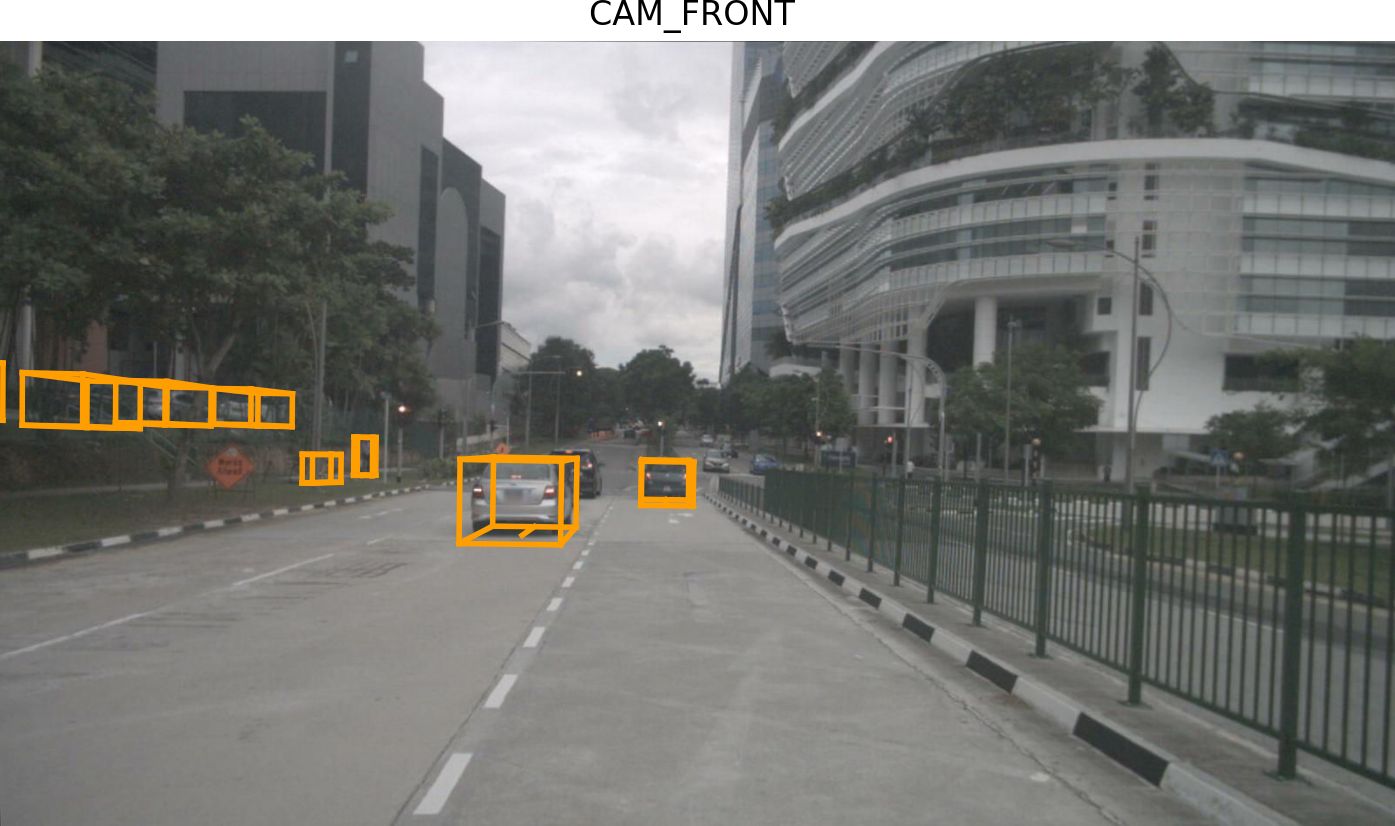
\includegraphics[width=0.31\columnwidth]{figure/visualize_predictions/GT-CAM_FRONT.png} & 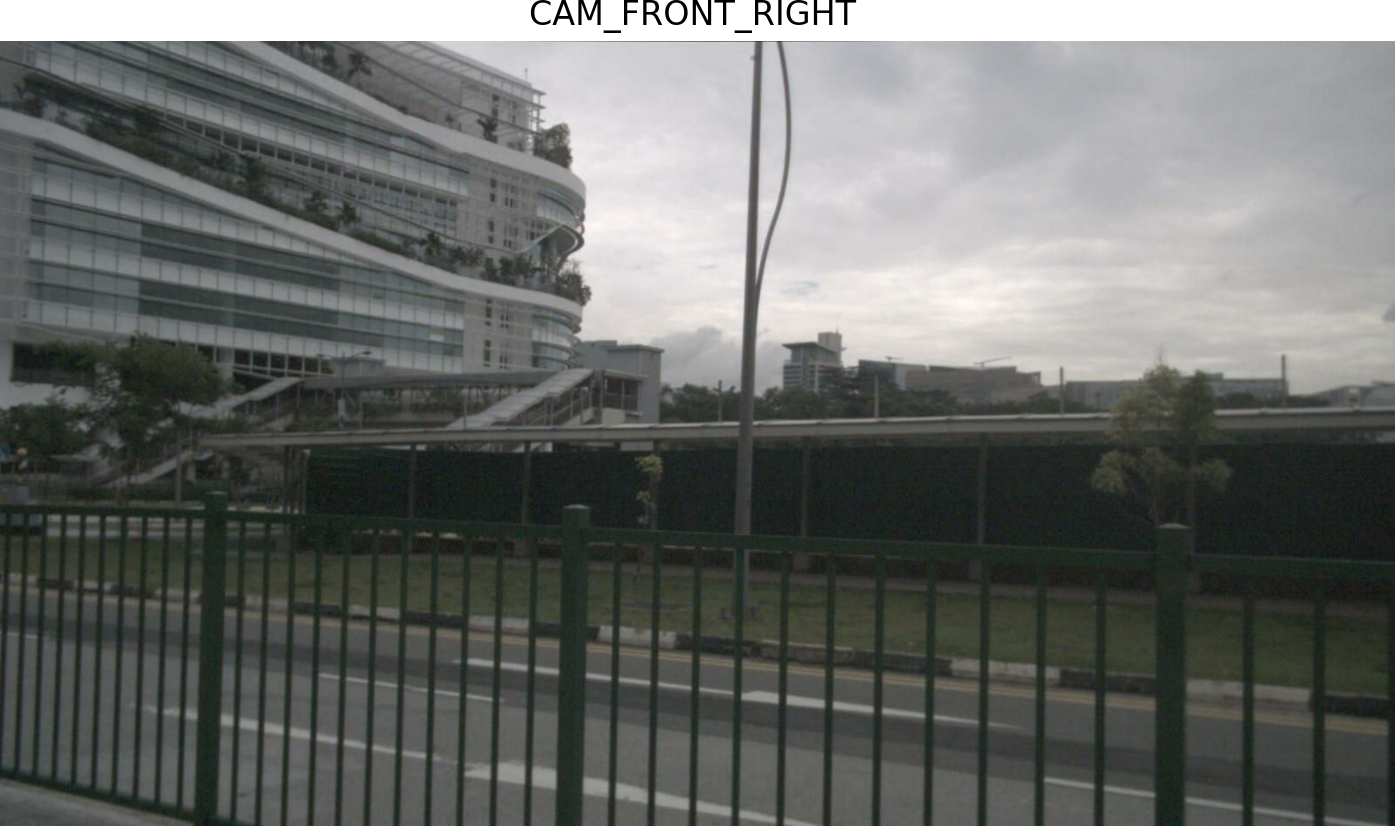
\includegraphics[width=0.31\columnwidth]{figure/visualize_predictions/GT-CAM_FRONT_RIGHT.png} \\ 
    \end{tabular}
    \end{minipage} \\
    
    \begin{minipage}{.27\textwidth}
        \begin{tabular}{@{}p{1em}@{}c@{}}
        \rotatebox{90}{\small{真值}} & \includegraphics[width=1.0\textwidth]{figure/visualize_predictions/GT-LIDAR_TOP.png}
    \end{tabular}
    \end{minipage}
    & 
    \begin{minipage}{.73\textwidth}
        \begin{tabular}{@{}p{1em}@{}c@{}c@{}c@{}}
        \rotatebox{90}{\small{预测}} &
    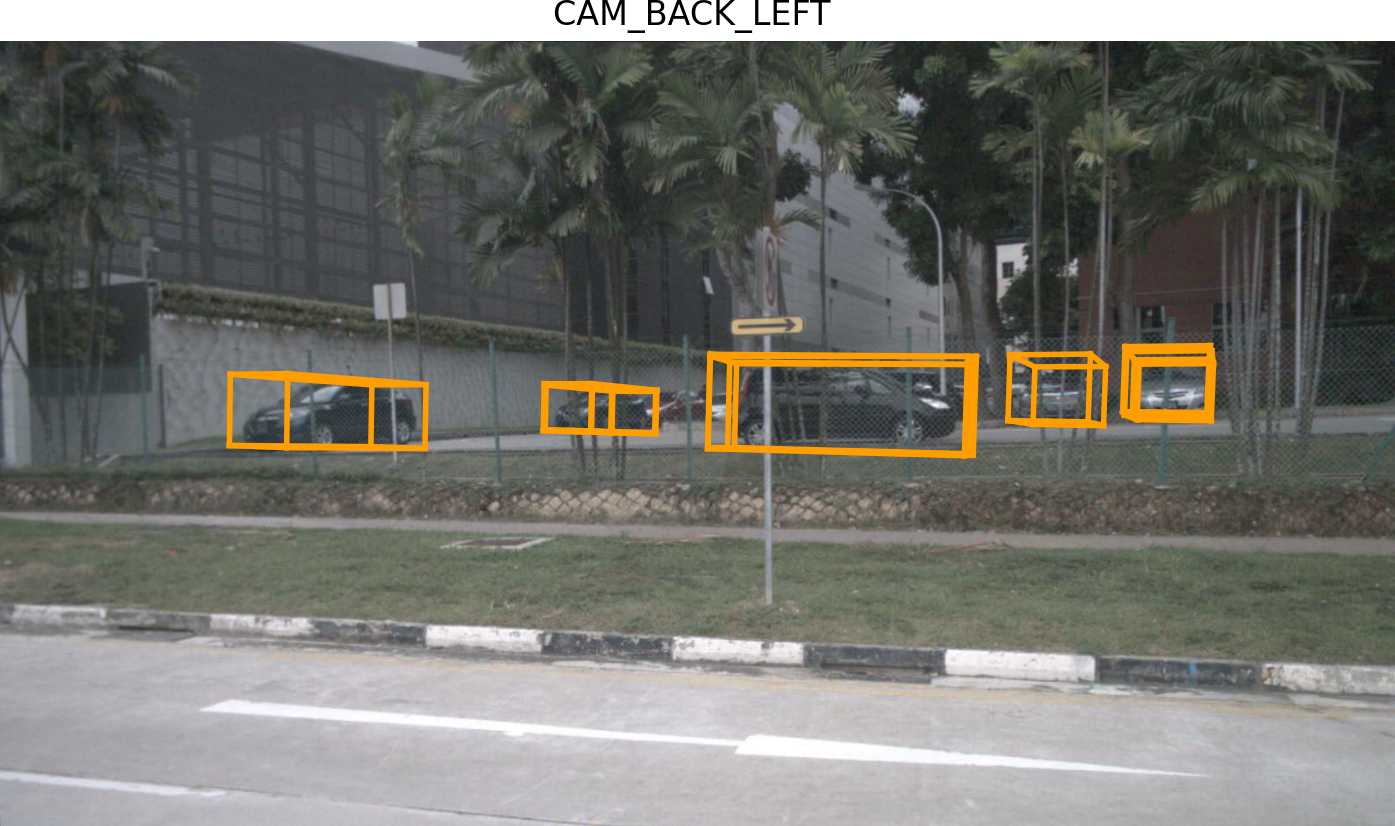
\includegraphics[width=0.31\columnwidth]{figure/visualize_predictions/CAM_BACK_LEFT.png} & 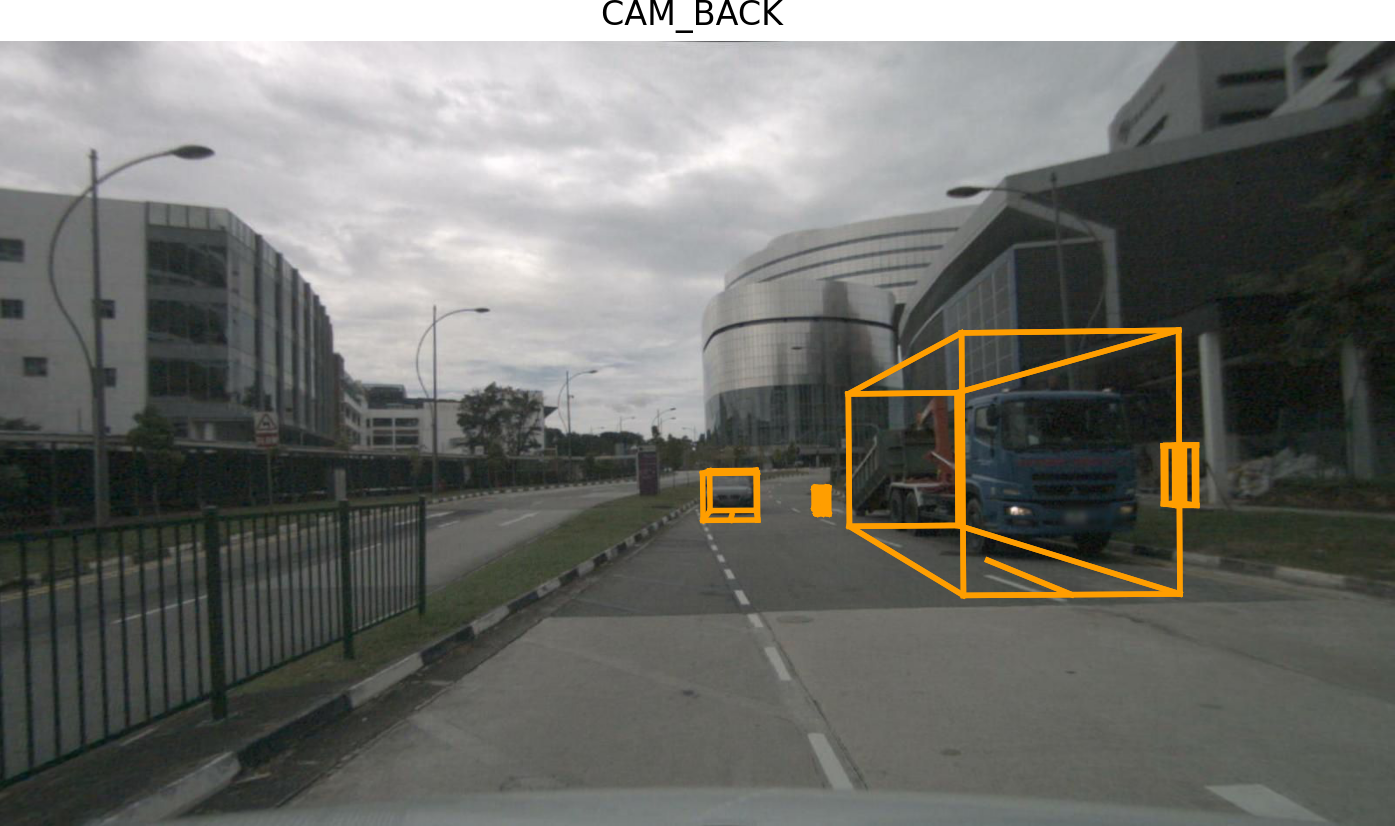
\includegraphics[width=0.31\columnwidth]{figure/visualize_predictions/CAM_BACK.png} & 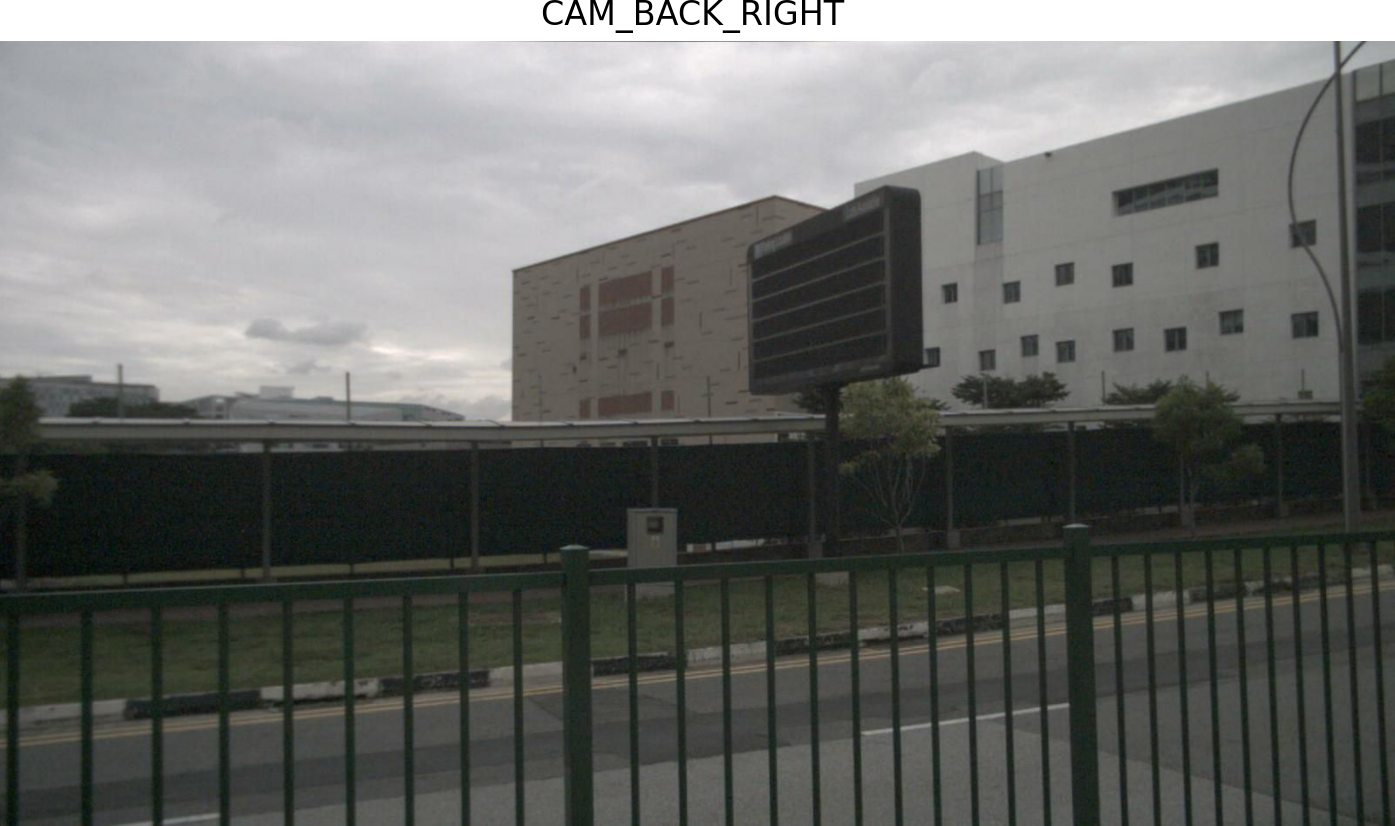
\includegraphics[width=0.31\columnwidth]{figure/visualize_predictions/CAM_BACK_RIGHT.png} \\ 
            \rotatebox{90}{\small{真值}} &
    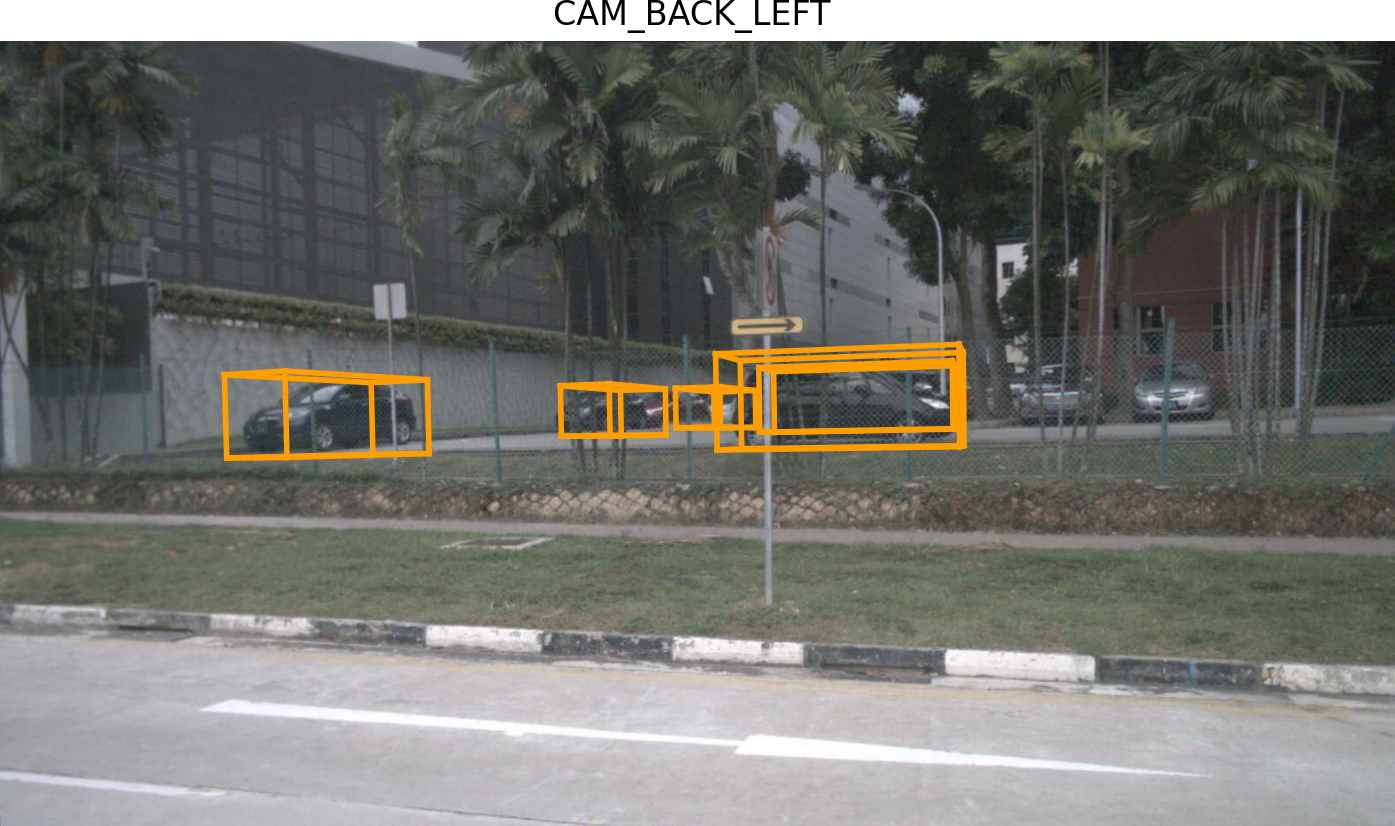
\includegraphics[width=0.31\columnwidth]{figure/visualize_predictions/GT-CAM_BACK_LEFT.png} & 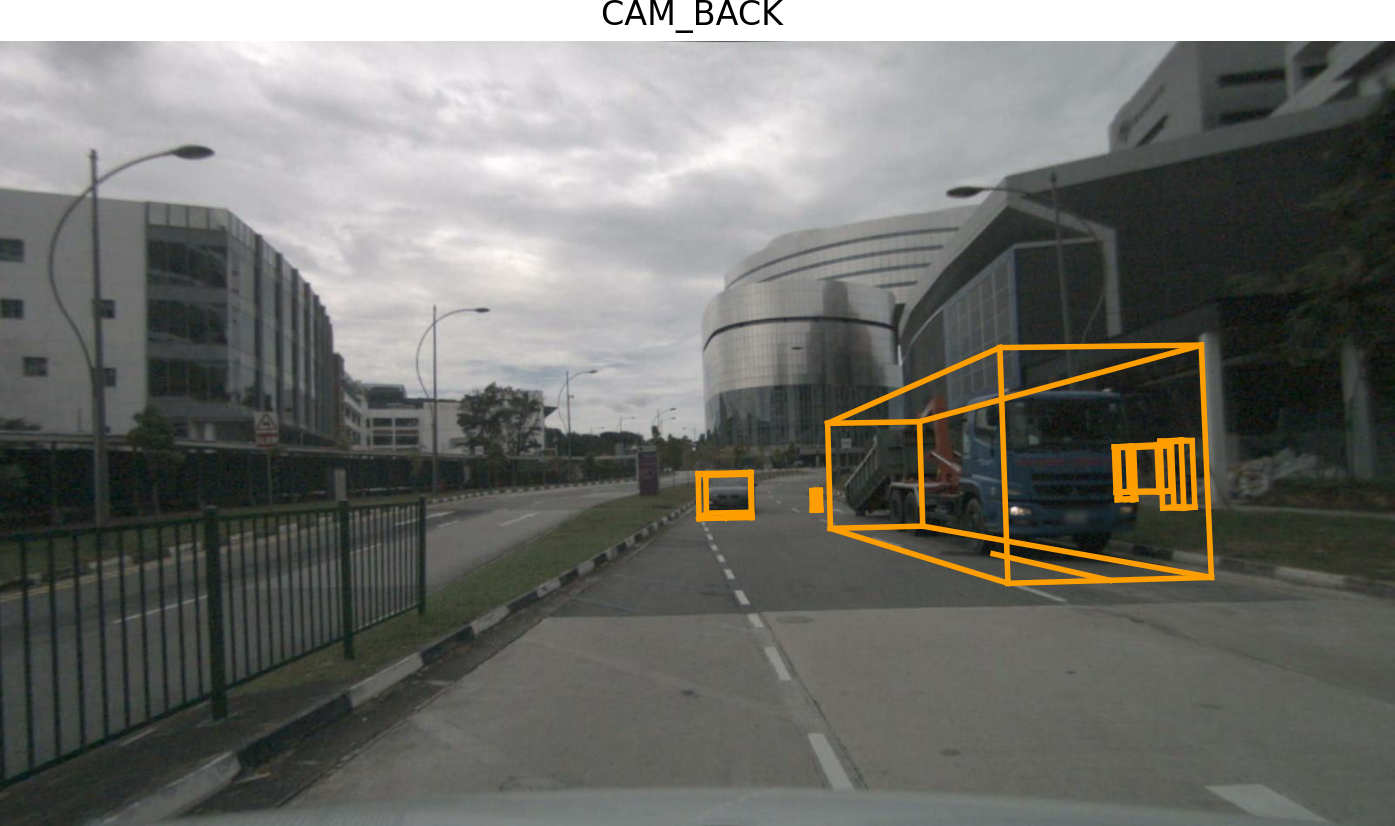
\includegraphics[width=0.31\columnwidth]{figure/visualize_predictions/GT-CAM_BACK.png} & 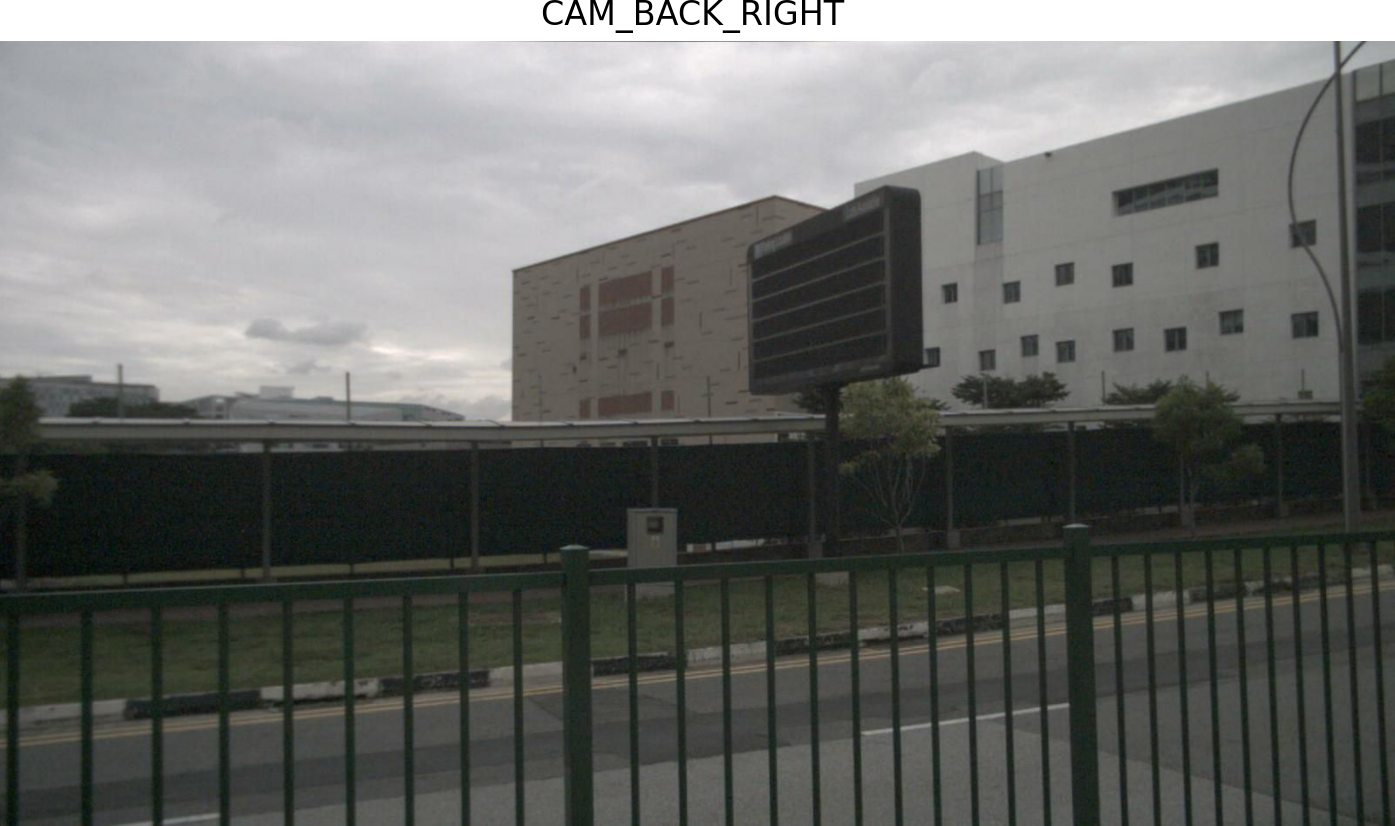
\includegraphics[width=0.31\columnwidth]{figure/visualize_predictions/GT-CAM_BACK_RIGHT.png} \\ 
    
        \end{tabular}
    \end{minipage} \\
    % \multirow{ 2}{*} 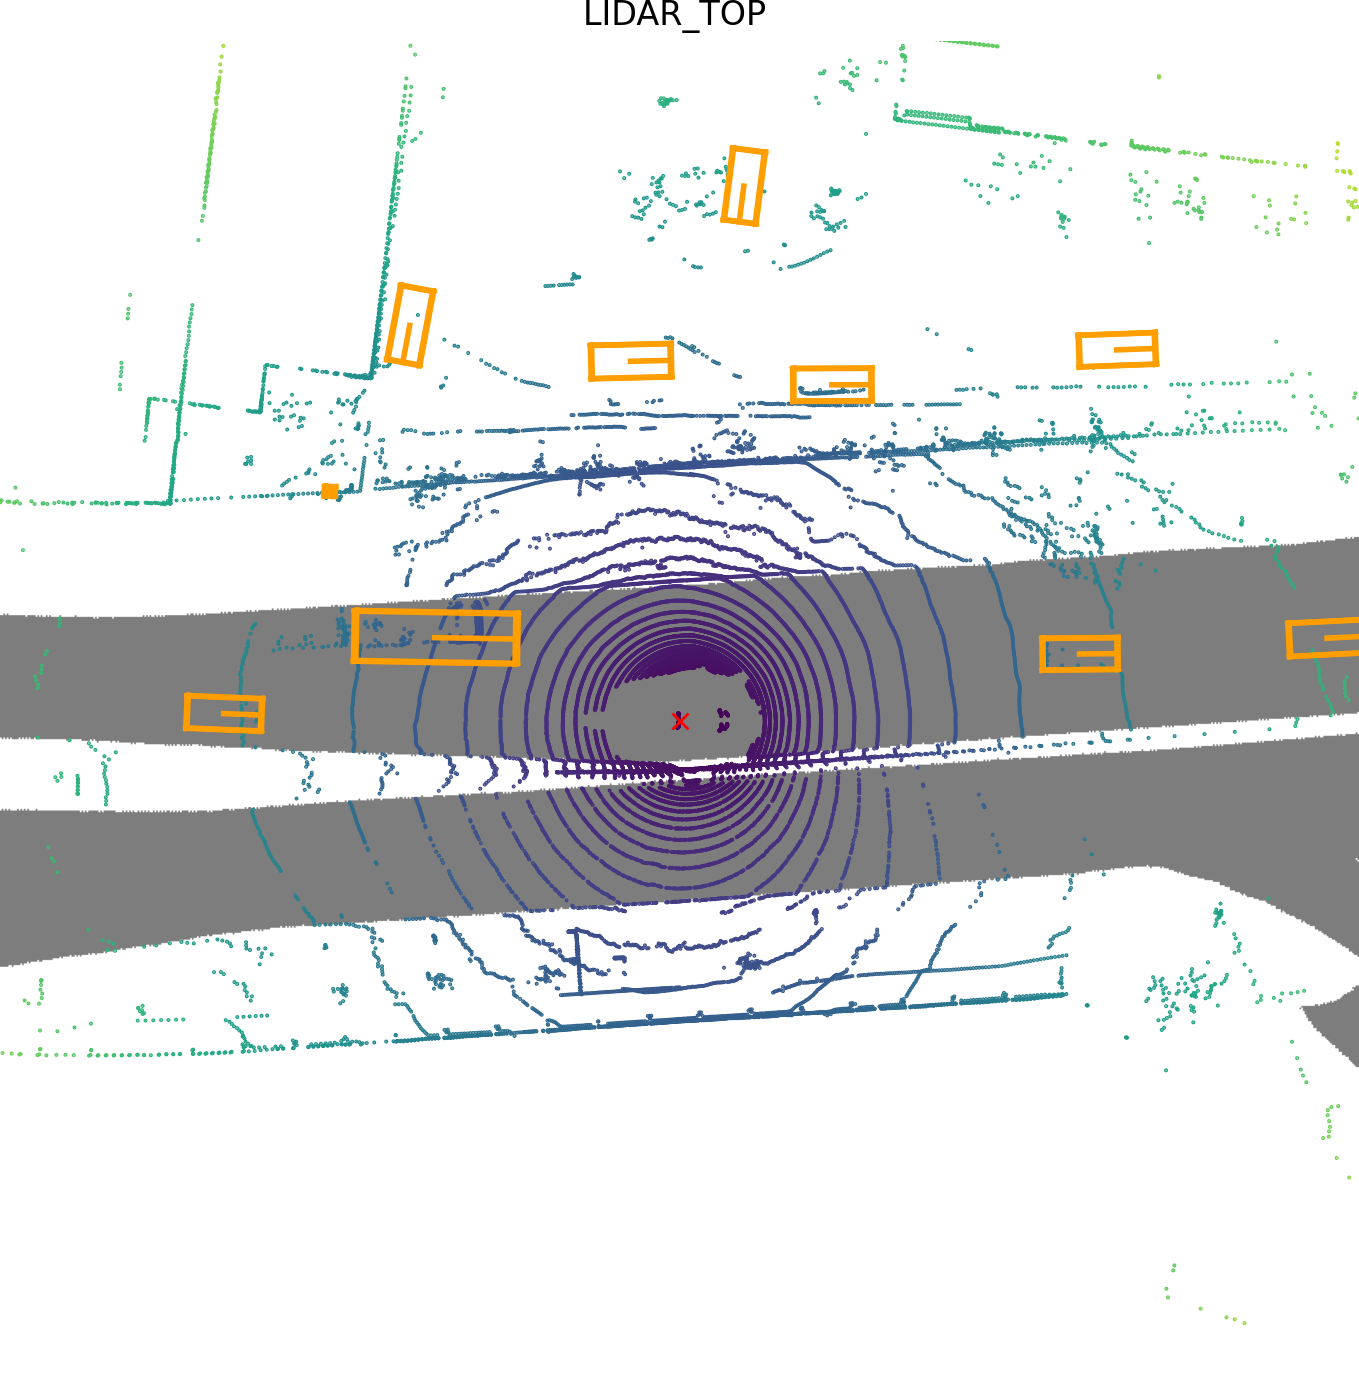
\includegraphics[width=0.3\columnwidth]{figure/visualize_predictions/LIDAR_TOP.png} & 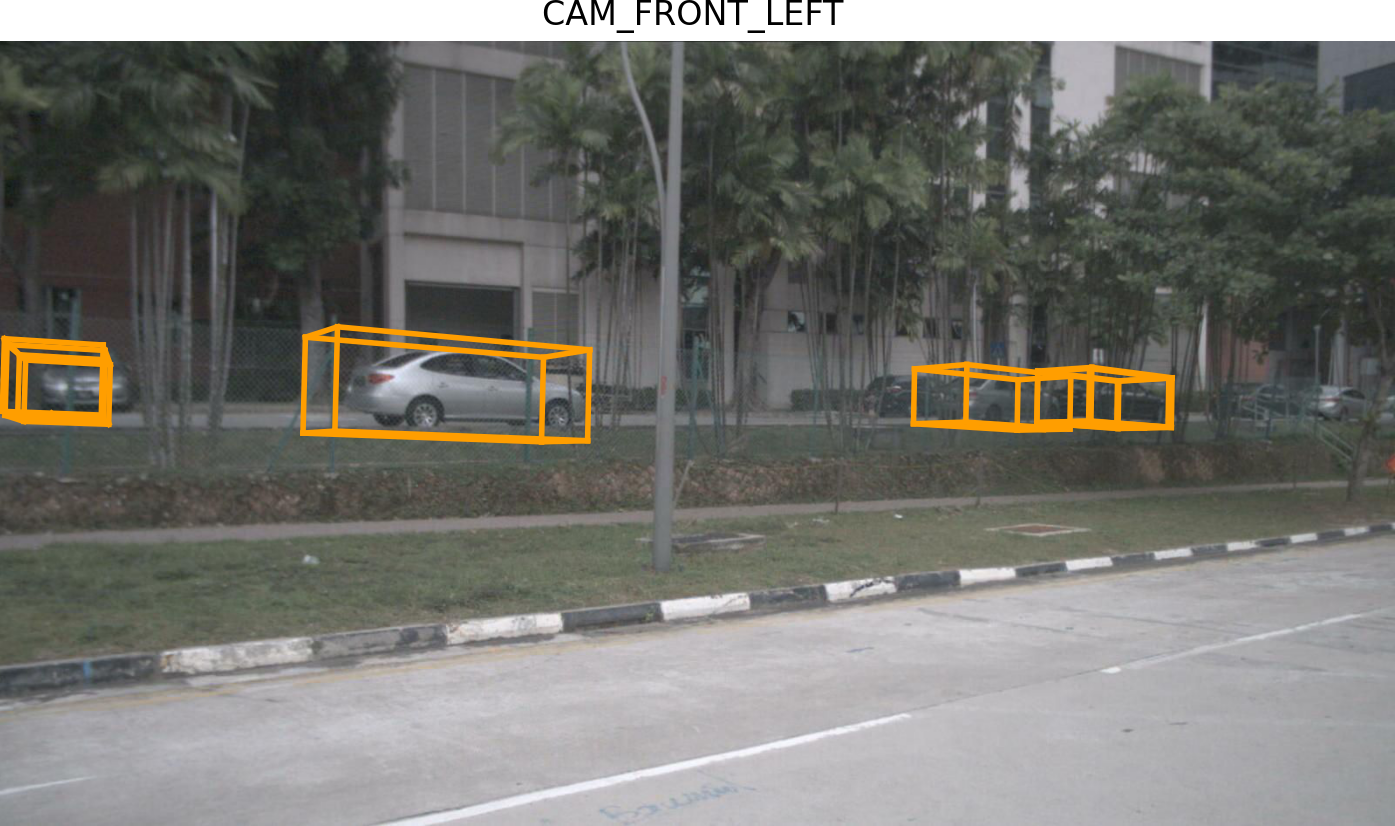
\includegraphics[width=0.3\columnwidth]{figure/visualize_predictions/CAM_FRONT_LEFT.png} & 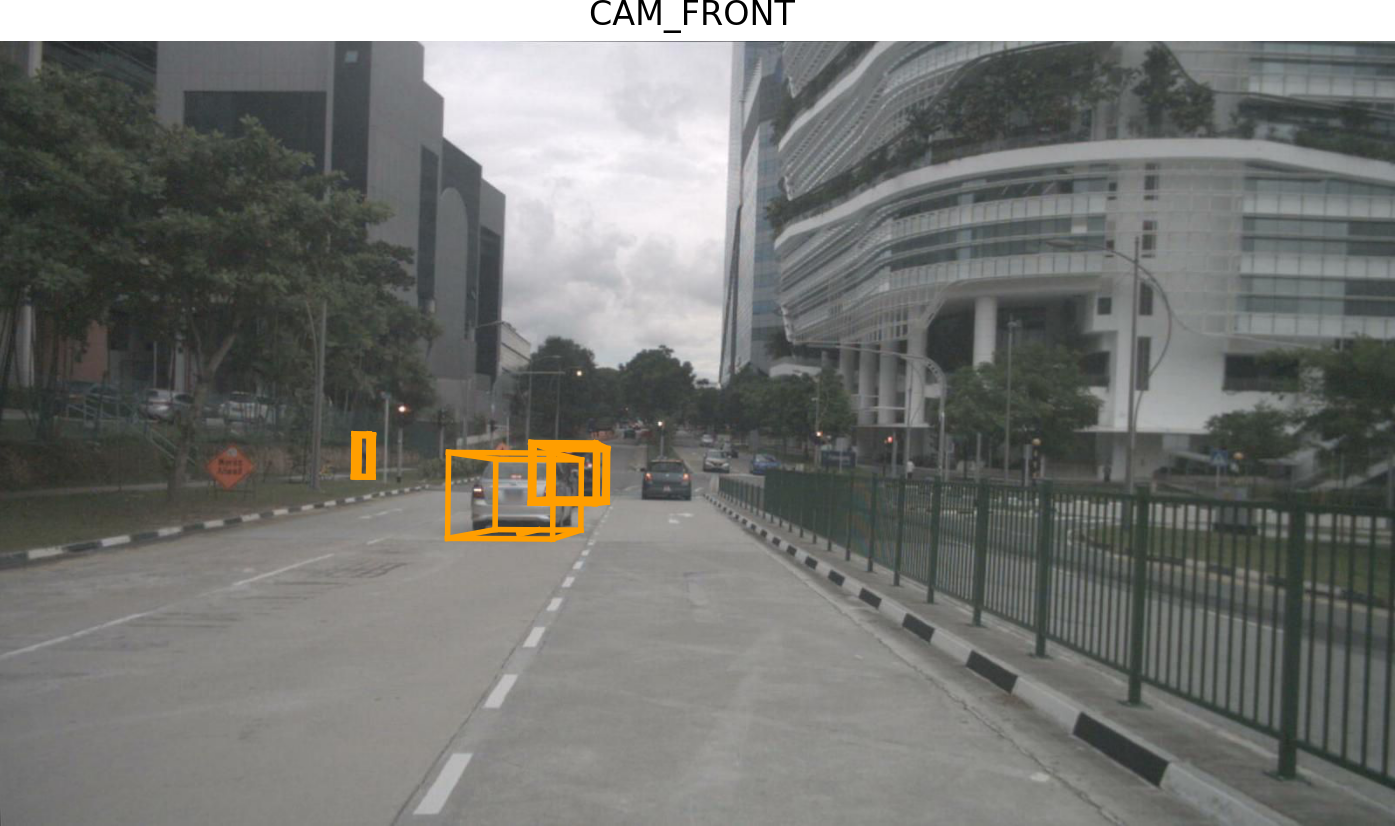
\includegraphics[width=0.3\columnwidth]{figure/visualize_predictions/CAM_FRONT.png} & 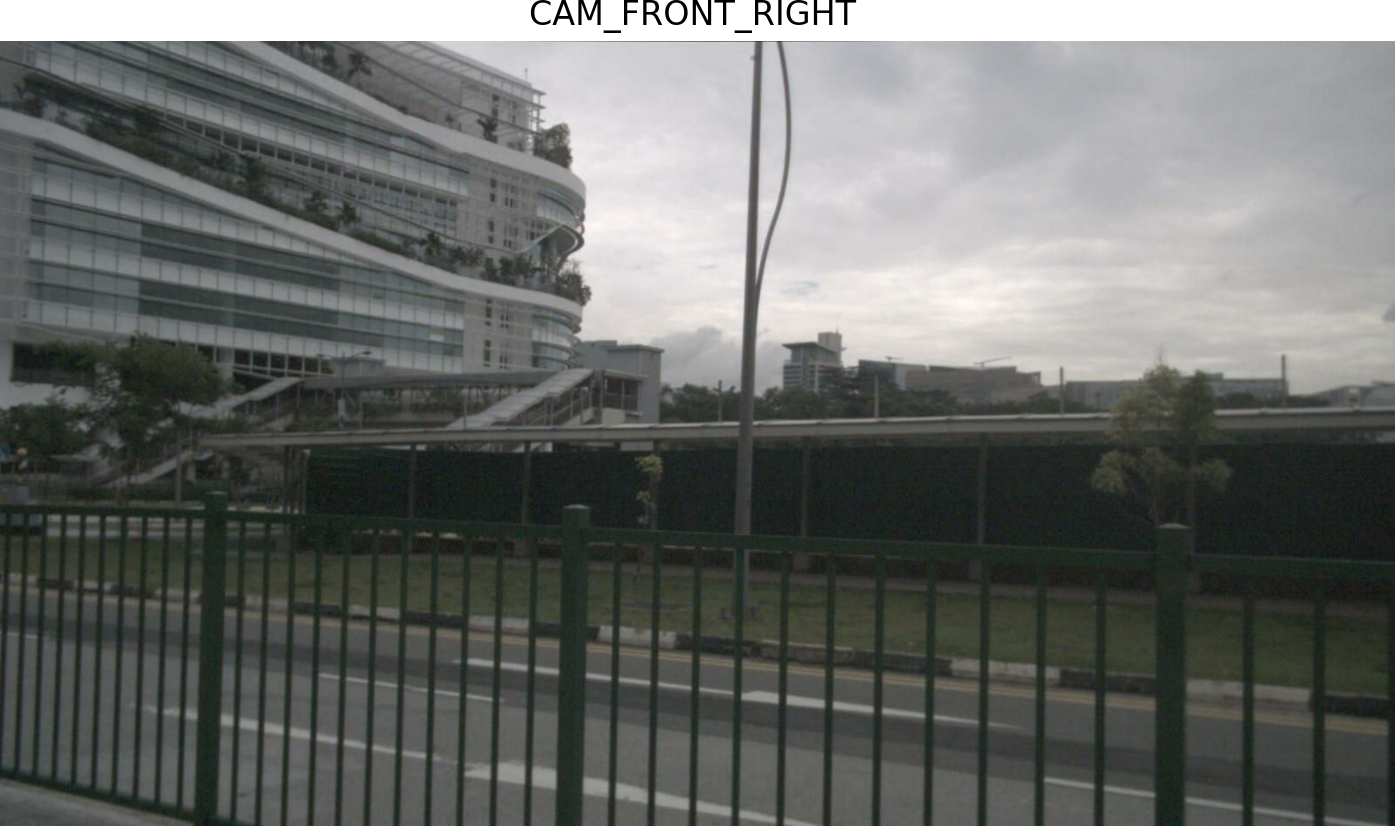
\includegraphics[width=0.3\columnwidth]{figure/visualize_predictions/CAM_FRONT_RIGHT.png} \\ 
    % & 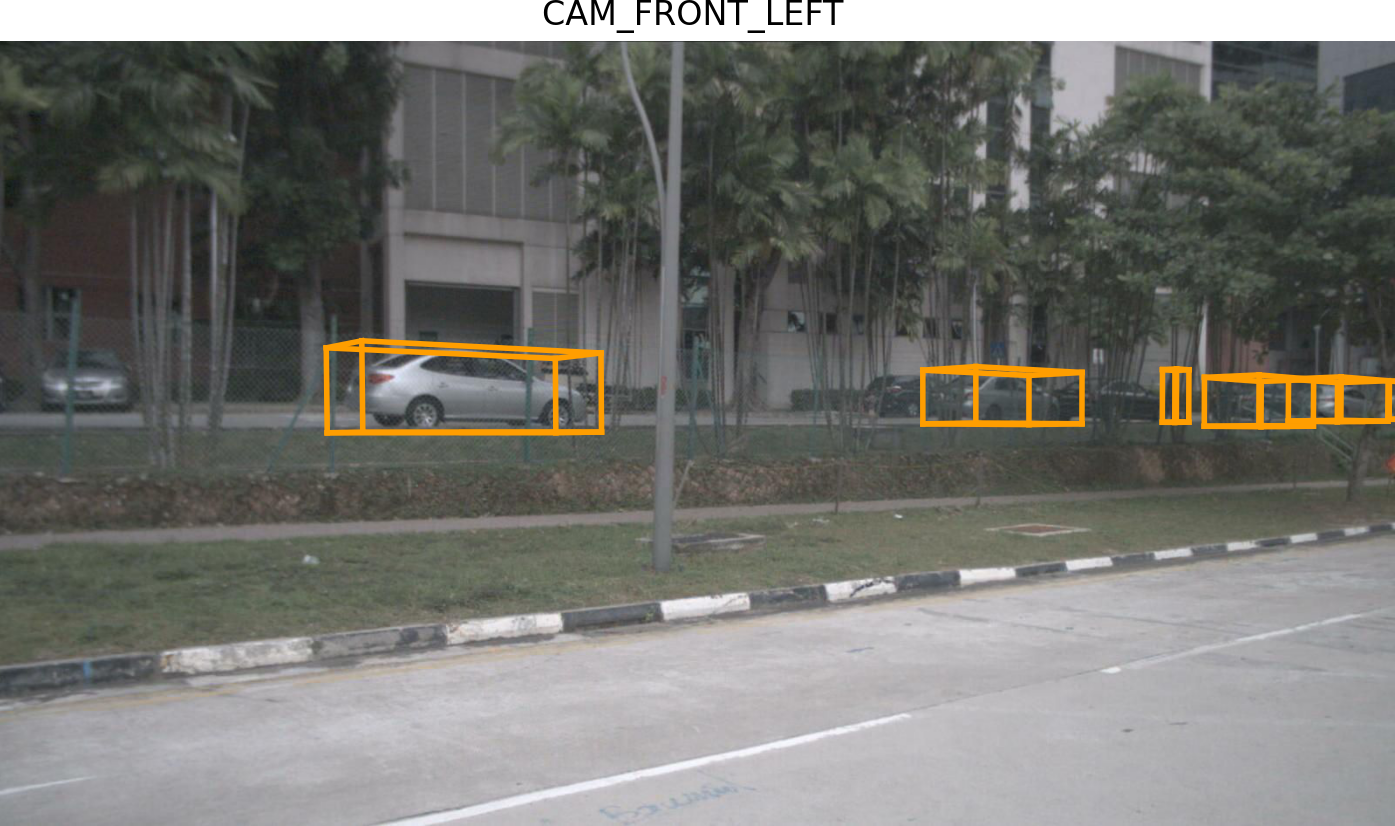
\includegraphics[width=0.3\columnwidth]{figure/visualize_predictions/GT-CAM_FRONT_LEFT.png} & 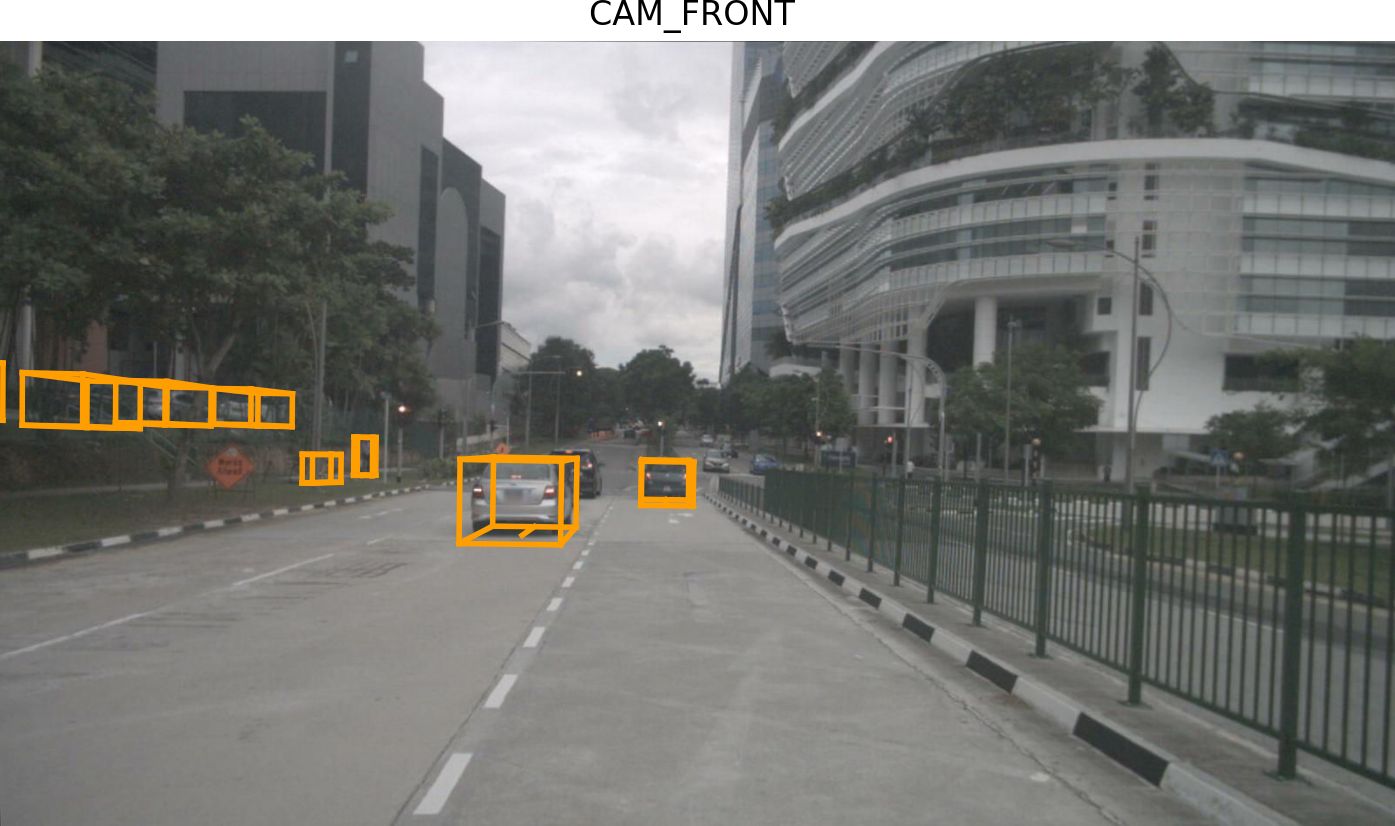
\includegraphics[width=0.3\columnwidth]{figure/visualize_predictions/GT-CAM_FRONT.png} & 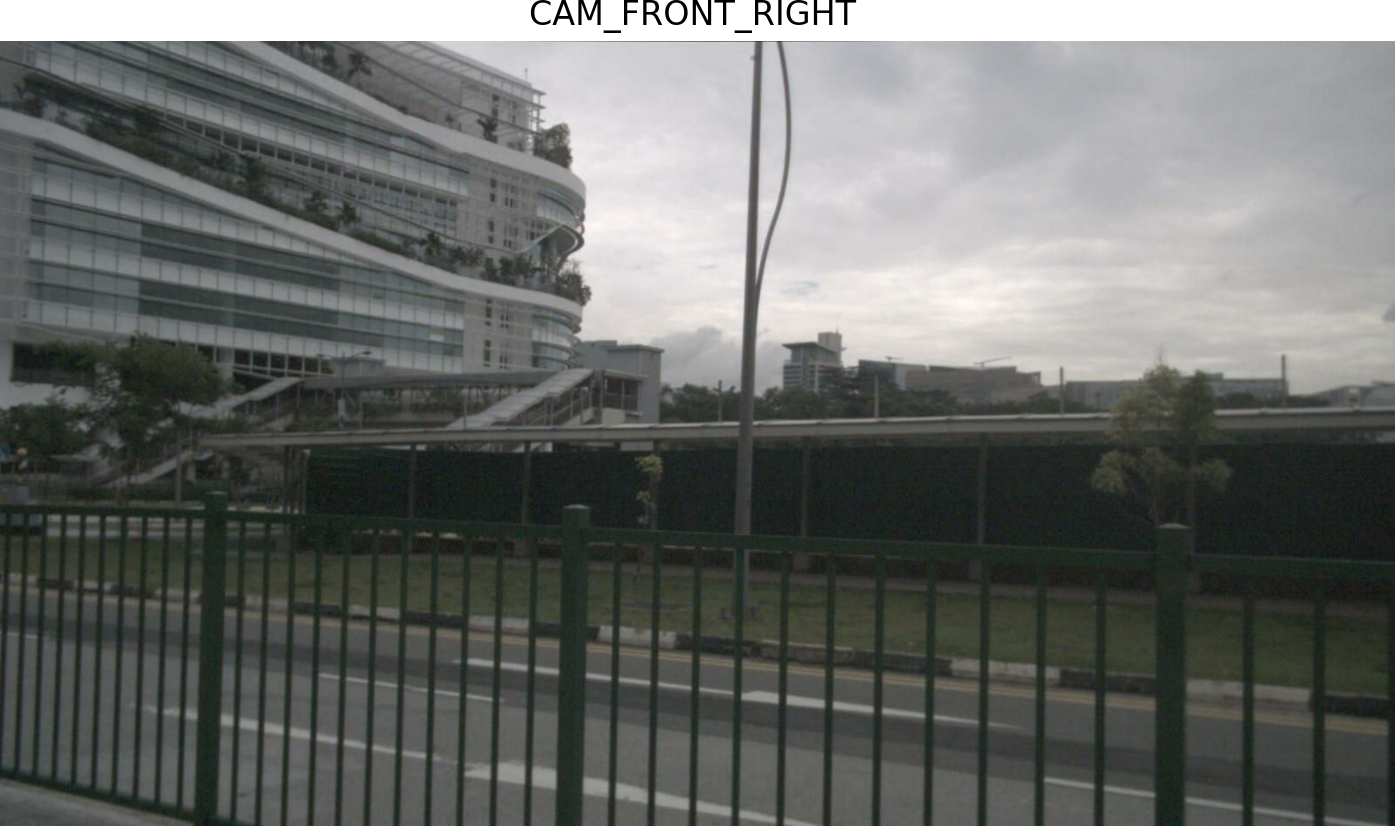
\includegraphics[width=0.3\columnwidth]{figure/visualize_predictions/GT-CAM_FRONT_RIGHT.png} \\ 
    \end{tabular}
  \caption{\name 预测结果的可视化，包括BEV和图像视图。本文模型能够检测相当小的目标，甚至包括未标注为真值的目标（\texttt{CAM\_BACK\_LEFT}中的车辆）。一些失败案例包括\texttt{CAM\_FRONT}中远处的车辆未被检测到。\label{fig:prediction}}
%   \vspace{-3em}
\end{figure}
% \end{comment}

%  Moreover, Table~\ref{sota} shows our method exhibits high translation error, which we suspect is due to the reference point parameterization; seeking better reference point parameterization can potentially increase the performance. 

% 1. Backbone of different sizes
% 2. Level, cam embedding


% Better Scene Prior: evaluate
% \begin{itemize}
%     \item Overlapping objects
%     \item What if one camera fails (low priority)
% \end{itemize}





% \subsection{Visualization}
% Visualize Ours backward
% \begin{itemize}
%     \item Reference points in 3d Scenes.  iterative refine process
%     \item Visualization feature fuse process (mask)
% \end{itemize}

% Visualization of Forward methods

% \begin{itemize}
%     \item Lift all pixels.
% \end{itemize}



